% SPDX-FileCopyrightText: 2023 SAP SE
%
% SPDX-License-Identifier: Apache-2.0
%
% This file is part of FEDEM - https://openfedem.org

%%%%%%%%%%%%%%%%%%%%%%%%%%%%%%%%%%%%%%%%%%%%%%%%%%%%%%%%%%%%%%%%%%%%%%%%%%%%%%%%
%
% FEDEM User Guide.
%
%%%%%%%%%%%%%%%%%%%%%%%%%%%%%%%%%%%%%%%%%%%%%%%%%%%%%%%%%%%%%%%%%%%%%%%%%%%%%%%%

\Chapter{Postprocessing Results}{postprocessing-results}

This chapter introduces the options for postprocessing the results calculated by
the various Fedem solvers.
You will learn how to set up graphs, curves and animations.

Sections in this chapter address the following topics:

\begin{itemize}
\item
  \protect\hyperlink{postprocessing-environment}
                    {Postprocessing environment}
\item
  \protect\hyperlink{graphs}
                    {Graphs}
\item
  \protect\hyperlink{beam-diagrams}
                    {Beam diagrams}
\item
  \protect\hyperlink{graph-groups}
                    {Graph groups}
\item
  \protect\hyperlink{animations}
                    {Animations}
\item
  \protect\hyperlink{viewing-animations}
                    {Viewing animations}
\end{itemize}

\clearpage


%%%%%%%%%%%%%%%%%%%%%%%%%%%%%%%%%%%%%%%%%%%%%%%%%%%%%%%%%%%%%%%%%%%%%%%%%%%%%%%%
\Section{Postprocessing environment}{postprocessing-environment}

In Fedem, postprocessing means evaluating the data collected from the mechanism
analysis (see \refChapter{mechanism-analysis}{Mechanism Analysis}).
The options for postprocessing are graphing and animating.
You can perform these tasks using the {\sl Results} list of the Model Manager
panel and the commands available in the \textbf{Result} menu.
Results are displayed in the Workspace area.

\medskip\noindent
\begin{minipage}{0.64\textwidth}
  \raggedright
  \subsubsection{Manager Results list}

  The {\sl Results} list of the Model Manager panel (shown at right)
  displays the list of user-defined result views in the model.
  In addition to the commands available in the
  \protect\hyperlink{result-menu}{\sl Result menu} (see below), many shortcut
  commands can be used to manage results in the {\sl Results} list.
  The shortcut menu, which is accessed by right-clicking in the Model Manager
  panel, displays commands relevant for the selected object only.

  \vskip\baselineskip
  Each curve object in the Model Manager {\sl Result} list has an icon next to
  the curve name, representing its legend. The curve color and symbol can be
  changed in the {\sl Appearance} tab (see \refSection{appearance}{Appearance}).
\end{minipage}%
\hfill\begin{minipage}{0.28\textwidth}
  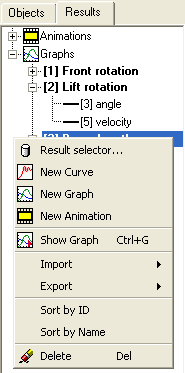
\includegraphics[width=\textwidth]{Figures/7-RightClickMenuInResultsList}
\end{minipage}

\medskip\noindent
\begin{minipage}{0.5\textwidth}
  \raggedright
  \SubSubSection{Result menu}{result-menu}

  The \textbf{Result} menu (shown at right) contains commands for creating
  result views, and managing the result files in your model.
  Use of these commands is explained in the following sections.

  \subsubsection{Workspace area}

  The Workspace area is used to display the graphs and animations you create.
\end{minipage}%
\hfill\begin{minipage}{0.47\textwidth}
  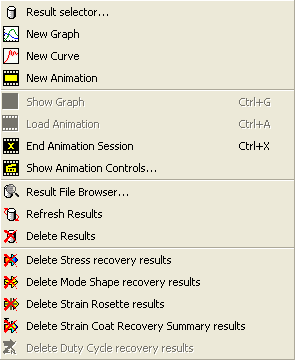
\includegraphics[width=\textwidth]{Figures/7-ResultMenu}
\end{minipage}

\begin{itemize}
\item
  Graphs can be displayed in individual windows that are labeled with the
  user-specified description of the graph; these windows are called {\sl Graph}
  views. To specify a description and display a {\sl Graph} view, see
  \refSection{graph-properties}{Graph properties} and
  \refSection{showing-a-graph}{Showing a graph}.
\item
  Animations can be displayed in the {\sl Modeler} view (one at a time).
  To display an animation, see
  \refSubSection{loading-animations}{Loading animations}{managing-animations}.
\end{itemize}


%%%%%%%%%%%%%%%%%%%%%%%%%%%%%%%%%%%%%%%%%%%%%%%%%%%%%%%%%%%%%%%%%%%%%%%%%%%%%%%%
\Section{Graphs}{graphs}

To track the progress of any variable during the simulation, you can create
two-dimensional graphs of the values. Each graph can contain several curves,
enabling comparison of the simulation variables.

\begin{center}
  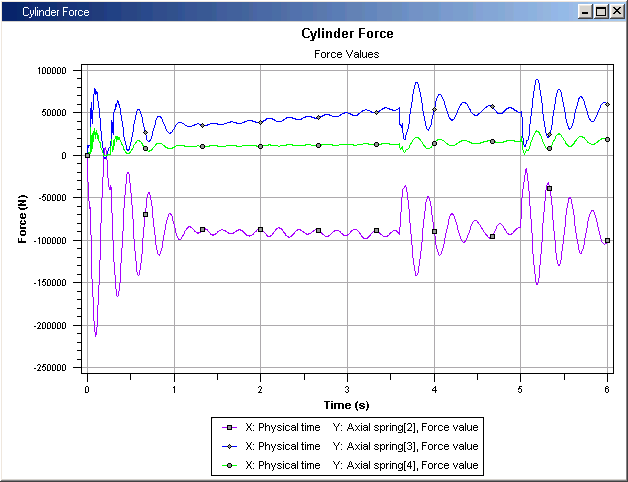
\includegraphics[width=0.9\textwidth]{Figures/Graph-view}
\end{center}

You can customize your graphs with titles, axis and data labels, and legends
(as shown below).

Graphs can be set up before or after performing the dynamics simulation.
If you create a graph before performing the simulation, you can observe
the values during the simulation, as they are constantly updated
(see \refSection{interaction-during-processing}{Interaction during processing}).
Otherwise, you can view the entire set of graphed values after the simulation
is completed.

Graphs plotting values vs. time will have a time indicator bar present when
a time history animation is loaded. This bar will show the current animation
time in the graph. This makes it easy to see the correlation between the motion
and the graphed values.

In addition to graphs plotting the evolution of result quantities during the
simulation, another type of graphs exists which plots the variation of a result
quantity along a beam structure at a certain time. These types of graphs
are described in \refSection{beam-diagrams}{Beam diagrams}.


\SubSection{Creating graphs and curves}{creating-graphs-and-curves}

You can create as many graphs as you like, either before or after doing the
dynamics simulation. It is recommended that you provide descriptive names for
your graphs, as the description is used in the Model Manager {\sl Results}
list to distinguish between graphs. The description is also used as the title
of the {\sl Graph} view when the graph is displayed in the Workspace area.
To specify a description, see \refSection{graph-properties}{Graph properties}.

Once you have created a graph, you will need to create curves (plotted data)
for the graph and specify descriptions and properties for the curves.

There are two ways to create these items, either by using the \textbf{New Graph}
and \textbf{New Curve} commands, or by dragging result variables from the RDB
selector dialog box into the {\sl Result} list of the Model Manager panel,
as described below.

\SubSubSection{Graph}{graph}

\IconTextFirst{createGraph}{
  To create a graph, select \textbf{New Graph} from the \textbf{Result} menu,
  or right-click in the Model Manager {\sl Results} list and select
  \textbf{New Graph}. An object titled ``New Graph'' is listed in
  the {\sl Results} list of the Model Manager panel.}

\subsubsection{Curves}

To create a curve, complete the following steps:

\vskip9mm
\IconText{createCurve}{\vspace*{-8mm}
  \begin{enumerate}
  \item
    In the Model Manager {\sl Results} list,
    select the graph to which you want to add the curve.
  \item
    Select \textbf{New Curve} on the {\sl Result} menu,
    or right-click the graph in the Model Manager {\sl Results} list and
    select \textbf{New Curve} there.
  \item
    Alternatively: Right-click an empty spot in the {\sl Results} list of
    the Model Manager panel, and select \textbf{New Curve}.
    This will create a new graph with a single curve.
  \end{enumerate}}

An object named ``New Curve'' is then listed under the current graph in the
{\sl Results} list of the Model Manager panel.

\SubSubSection{Creating curves and graphs by drag and drop}
              {creating-curves-and-graphs-by-drag-and-drop}

\noindent
\begin{minipage}{0.58\textwidth}
  \raggedright
  When you need to create several curves and graphs containing results from the
  results database, or want to inspect several result values without the need to
  create persisting graphs for all of them, it is convenient to use the drag and
  drop method to create and sort curves and graphs.

  \vskip\baselineskip
  To create curves or graphs by drag and drop, right-click in the {\sl Result}
  list of the Model Manager panel and select \textbf{Result selector...}
  The RDB selector dialog box then pops up (shown to the right).

  \vskip\baselineskip
  Select the result you want to plot, and drag it from the RDB selector dialog
  box and onto the {\sl Result} list of the Model Manager panel. If you drop it
  on an existing graph, it will be created as a curve in that graph, otherwise
  a new graph will be created with the selected results as a new curve.

  \vskip\baselineskip
  If the graph receiving the new curve is visible,
  the new data is automatically loaded and displayed.

  \vskip\baselineskip
  For more detailed information about the RDB selector dialog box, see
  \refSubSection{selecting-rdb-results}{Selecting RDB results}
                {curve-properties}.
\end{minipage}
\hfill\begin{minipage}{0.4\textwidth}
  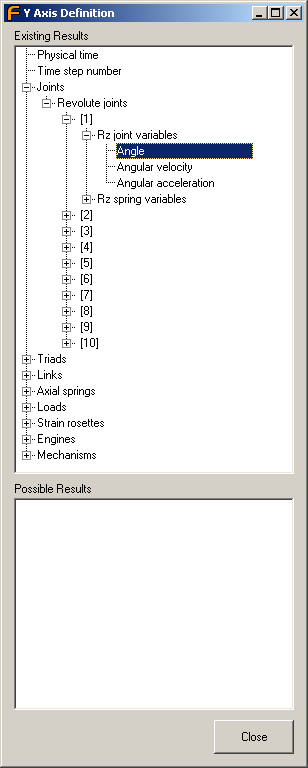
\includegraphics[width=\textwidth]{Figures/Dialogs/7-RDB-Selector-DragAndDrop}
\end{minipage}

\subsubsection{Repeat a curve definition for all objects}

In some cases it is useful to look at some particular result from all objects
of a certain type in the model. E.g., to find the triad with the highest forces
in the model, or to look at the acceleration levels all over the model.

\IconText{repeatCurve}{
  This can be achieved in a convenient way using the command labeled
  \textbf{Repeat curve for all objects}. This command is available in the
  right-click menu of the {\sl Result} list of the Model Manager panel,
  when right-clicking a curve. This command repeats the curve definition
  of the curve selected, and uses it on all the objects of the same type
  in the model. It also automatically assigns a color to the curves
  depending on the ID number of the object. The colors assigned will be
  black-blue-cyan, where low ID numbers makes the curve get a black-ish color,
  while higher numbers will turn the curve blue or cyan.}

Normally, it is only the object used for the $Y$-axis value in the curve
definition that is cycled, but if the curve being repeated uses the same object
both for the $X$-, and $Y$-axis they are cycled together.

\begin{wrapfigure}[9]{r}{0.3\textwidth}
  \vspace{-5mm}
  \center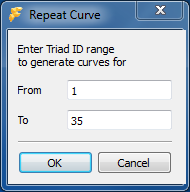
\includegraphics[width=0.3\textwidth]{Figures/Dialogs/7-RepeatCurveForRange}
\end{wrapfigure}

It is also possible to repeat a curve definition for not every object of the
same type in the model, but only a subset of the similar objects. This is done
by using the command labeled \textbf{Repeat curve for object range...}
in the right-click menu of the {\sl Results} list of the Model Manager panel.
This opens a dialog box (shown to the right) where you can enter the user ID
range of the objects for which you want the curve definition to be repeated.

\Note{Since the user ID numbers are unique only within each sub-assembly
  (see \refSection{sub-assemblies}{Sub-assemblies}),
  the \textbf{Repeat curve for object range...} command applies only to the
  objects within the same sub-assembly as the object that is plotted by the
  selected curve. On the other hand, the \textbf{Repeat curve for all objects}
  command always applies to all objects in all sub-assemblies (if any)
  of the model.}

\subsubsection{Moving curves to a new graph}

To move curves from one graph to another, simply select the curves and
drag them to the new graph. This is done by pressing and holding the
left mouse button while the mouse cursor is above the curves to move,
then move the mouse to the target graph and release the mouse button.


\SubSection{Showing a graph}{showing-a-graph}

\IconTextFirst{showGraph}{
  To display graphs, select one or more graphs or curves in the Model Manager
  {\sl Results} list, right-click and select \textbf{Show Graph} on the shortcut
  menu (or select \textbf{Show Graph} on the \textbf{Result} menu). The selected
  {\sl Graph} views opens in the Workspace area displaying the graphs.}


\SubSection{Graph properties}{graph-properties}

Now that you can create a graph and its curves, you need to specify properties
for the graph. To display the properties in the Property Editor panel,
select the graph in the Model Manager {\sl Results} list.
The properties for the graph are displayed in the Property Editor panel
as shown below.

\noindent
\begin{picture}(343,100)
  \put(0,0){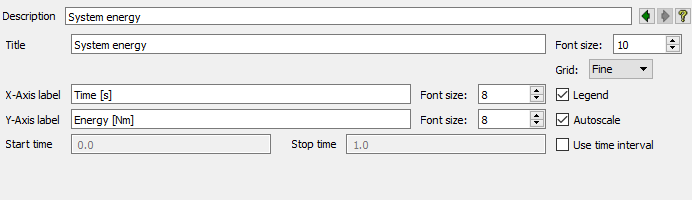
\includegraphics[width=\textwidth]{Figures/7-GraphProperty}}
  \put(75,86){\Bullet{1}}
  \put(80,73){\Bullet{2}}
  \put(80,48){\Bullet{3}}
  \put(80,35){\Bullet{4}}
  \put(315,72){\Bullet{5}}
  \put(325,60){\Bullet{6}}
  \put(305,47){\Bullet{7}}
  \put(310,36){\Bullet{8}}
  \put(325,22){\Bullet{9}}
\end{picture}

\begin{bulletlist}
\item{\sl Description} --
  An optional user-specified description that is displayed as both the graph
  name in the {\sl Results} list, and the title of the associated {\sl Graph}
  view in the Workspace area. It is recommended that you use a descriptive name
  or phrase to distinguish between similar graphs.
  This name is not included in the {\sl Graph} view itself.

\item{\sl Title} --
  You can specify a title for the graph
  that is displayed in the {\sl Graph} view.

\item{X-Axis Label} --
  You can provide a label for the abscissa
  that is displayed in the {\sl Graph} view.

\item{Y-Axis Label} --
  You can provide a label for the ordinate
  that is displayed in the {\sl Graph} view.

\item{Font size:} --
  You can specify the font size to be used on the legends and
  the axes tics marks in the {\sl Graph} view.

\item{\sl Grid} --
  You can specify the type of grid (coarse, fine, or no grid)
  for the {\sl Graph} view by selecting from this pull-down menu.

\item{\sl Legend} --
  You can add a legend to the graph by enabling the {\sl Legend} option.
  The legend names you specify for each curve are used in the legend
  (see \refSection{curve-properties}{Curve properties} below).

\item{\sl Autoscale} --
  Enabling this option automatically scales the $X$- and $Y$-axes to accommodate
  new curves as they are added to the graph (or when opening the {\sl Graph}
  view). Disabling {\sl Autoscale} allows you to fully control the $X$- and
  $Y$-axis range.

\item{\sl Start time}, {\sl Stop time}, {\sl Use time interval} --
  You can enable the {\sl Use time interval} option to specify a time interval
  for loading the graph. Only the RDB data that fall within the specified time
  interval are loaded when the graph is opened or exported.
  This only affects curves that are plotting simulation results.
  Imported curves, or curves plotting an internal function are not affected by
  these settings.
\end{bulletlist}

\Note{When you make changes to graphs or curves in the Property Editor panel,
  the changes are updated dynamically in the graph view.}


\SubSection{Curve properties}{curve-properties}

Having completed the specification of a graph, you want to set the properties of
its associated curves. To display the curve properties in the Property Editor
panel, select the curve in the Model Manager {\sl Results} list.

The curve information is organized under six tabs, as shown below:
{\sl Data}, {\sl Appearance}, {\sl Curve Statistics}, {\sl Scale and Shift},
{\sl Fourier Analysis and Differentiation}, and {\sl Rainflow and Fatigue}.

The {\sl Data} tab is used to specify the data to be plotted and is described
below. The other five tabs are discussed in the subsequent sections.

\noindent
\begin{picture}(343,115)
  \put(0,0){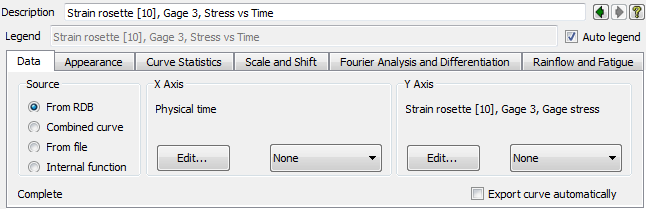
\includegraphics[width=\textwidth]{Figures/7-CurveProperty}}
  \put(150,100){\Bullet{1}}
  \put(142, 87){\Bullet{2}}
  \put( 35, 61){\Bullet{3}}
  \put(105, 61){\Bullet{4}}
  \put(230, 61){\Bullet{4}}
  \put(165, 22){\Bullet{5}}
  \put(295, 22){\Bullet{5}}
  \put(235,  4){\Bullet{6}}
  \put(260, 80){\Bullet{7}}
  \put(160, 80){\Bullet{8}}
  \put( 60, 80){\Bullet{9}}
  \put(110, 80){\BBullet{10}}
  \put(330, 80){\BBullet{11}}
\end{picture}

\begin{bulletlist}
\item{\sl Description} --
  This is the name of the curve in the Model Manager {\sl Results} list.
  The description is updated automatically when changing the $X$- or $Y$-axis
  definitions, unless it has been edited manually in the mean time.
  This name is not used in the {\sl Graph} view.

  \EnumTip{If you have manually edited the description field of a curve,
    you can at any time return to the auto-generated description by
    deleting it completely.}

\item{\sl Legend} --
  If you choose not to supply a name for the curve, you can enable
  {\sl Auto legend} to use a combination of the $X$- and $Y$-axis labels for the
  legend. When {\sl Auto legend} is used, the legend will always be equal to the
  auto-generated description of the curve.

  \EnumNote{The {\rm Legend} option must be enabled in the Graph Property Editor
    panel to display the legend in the {\rm Graph} view
    (see \refSection{graph-properties}{Graph properties}).}

\item{\sl Source} --
  The data plotted in a curve originate either from the results database
  ({\sl From RDB}), from an external file ({\sl From file}),
  or from a Fedem function ({\sl Internal function}).
  In addition, the data can be defined via a mathematical expression
  with some of the other curves as variables ({\sl Combined curve}).
  The Property Editor panel shown above is that of a {\sl From RDB} curve.
  The panels of the other curve types are discussed below (see
  \protect\hyperlink{creating-curves-from-file}
                    {\sl"Creating curves from file"},
  \protect\hyperlink{creating-curves-from-a-function}
                    {\sl"Creating curves from a function"}, and
  \protect\hyperlink{creating-combined-curves}
                    {\sl"Creating combined curves"} below).

\item{\sl X Axis}, {\sl Y Axis} --
  To define the values used for the $X$- and $Y$-axes in a {\sl From RDB} curve,
  click the \textbf{Edit...} button. The RDB selector dialog box is then opened
  allowing you to pick the wanted results (see
  \protect\hyperlink{selecting-rdb-results}{\sl"Selecting RDB results"}
  below for details). Alternatively, one may also right-click a curve in the
  Model Manager {\sl Results} list and then select \textbf{Edit X Axis...}
  or \textbf{Edit Y Axis...}

  \EnumTip{While editing the $x$-axis, you can click \textbf{Apply} in the RDB
    selector dialog box, then click the \textbf{Edit...} button for the $y$-axis
    and start selecting result quantitiy for that axis.}

\item{\sl Result Operation} --
  The pull-down menus next to the \textbf{Edit...} buttons list mathematical
  operations (such as extracting the $X$-component or computing the length of a
  vector) related to the result quantities selected for the $X$- and $Y$-axis.
  If the result quantity selected in Step 4 above is a {\sl Position matrix}
  (of either a Triad or Part), the menu will also contain several angular
  quantities which can be derived from the position matrix. See
  \protect\hyperlink{derived-angular-quantities-from-position-matrices}
                    {\sl"Derived angular quantities from position matrices"}
  below for further details on these items.

  \EnumNote{If you make a change to the {\rm Result Operation} choice,
    the curve changes dynamically in the graph view.}

\item{\sl Export curve automatically} --
  Toggles whether the dynamics solver shall export this curve automatically,
  to the file specified in the Dynamics Solver Setup dialog box.
  See \refSubSection{output-tab}{Output tab}{dynamics-solver-advanced-mode}.

\item{\sl Fourier Analysis and Differentiation} -- This tab
  allows you to perform a Fast Fourier Transformation of the curve data. See
  \refSection{fourier-analysis-differentiation-and-integration}
             {Fourier analysis, differentiation and integration}. You may
  also plot the derivative or the integral of the curve data via this tab.

\clearpage
\item{\sl Scale and Shift} --
  This tab allows you to apply scaling and shift to the curve data.
  See \refSection{scale-and-shift}{Scale and Shift}.

\item{Appearance} --
  This tab allows you to change appearance of individual curves.
  See \refSection{appearance}{Appearance}.

\item{\sl Curve Statistics} --
  This tab allows you to extract statistical properties for individual curves.
  See \refSection{curve-statistics}{Curve Statistics}.

\item{\sl Rainflow and Fatigue} --
  This tab allows you to perform a Rainflow calculation and to assess fatigue
  results based on the curve data. See
  \refSection{fatigue-calculation}{Fatigue calculation from standard S-N curves}.
\end{bulletlist}

\Note{The curve is not displayed in the graph view until you have fully defined
  the curve variables (indicated by the word {\rm"Complete"} appearing at the
  bottom of the Property Editor panel).
  The word {\textcolor{red}\rm"Incomplete"} appears at the same location
  until the curve is properly defined.}

\Tip{Once you have created and fully defined curves, you can select them
  directly in the {\rm Graph} view, or clicking a curve in the {\rm Results}
  list of the Model Manager panel.
  When selected, curves are highlighted in red.}

\Tip{You can drag a curve object from one graph object and drop into another
  in the Model Manager {\rm Results} list.}

\clearpage

\SubSubSection{Selecting RDB results}{selecting-rdb-results}

\begin{minipage}{0.64\textwidth}
  \raggedright
  To select the results to plot as $x$- and $y$-axis values for a curve,
  complete the following steps:

  \medskip
  \begin{enumerate}
    \setlength\itemsep{1mm}
  \item
    In the Model Manager {\sl Results} list, select the curve you want to edit.
    Its properties are displayed in the Property Editor panel.
  \item
    In the Property Editor panel, click the \textbf{Edit...} button for the
    {\sl X-Axis}, or right-click on a curve in the Model Manager {\sl Results}
    list and select \textbf{Edit X Axis...} or \textbf{Edit Y Axis...}.
    The RDB selector dialog box (shown at right) is then opened.
  \item
    Select a mechanism element from the {\sl Existing Results} list or in the
    {\sl Modeler} view.
    \vskip1mm
    \MiniGenericNote{note}{NOTE}{-30mm}{1.72}{0.17}{0.5}{
      If the mechanism analysis have been performed, variables for the
      selected element are listed in the {\rm Existing Results} list.
      If you have not yet performed an analysis, variables are listed in the
      {\rm Possible Results} list.}
  \end{enumerate}
\end{minipage}%
\hfill\begin{minipage}{0.35\textwidth}
  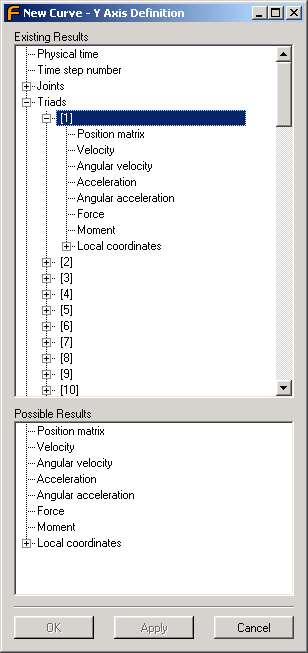
\includegraphics[width=\textwidth]{Figures/Dialogs/7-RDB-Selector}
\end{minipage}

\begin{enumerate}
\item[4.]
  Select a variable to be used as the $x$-axis quantity from either the
  {\sl Existing Results} or {\sl Possible Results} lists, and click \textbf{OK}
  to close the panel or \textbf{Apply} to continue variable selection.

  \EnumCaution{Some of the variables listed in the {\rm Possible Results}
    list may not be present in the results database.
    For example, a joint may or may not have a spring or damper attached at
    each DOF, but in the {\rm Possible Results} list all possible springs
    and dampers are listed -- one for each joint DOF.
    If such a nonexistent variable is selected, the associated curve does not
    appear in the graph view.}

  \EnumNote{Variables such as {\small\rm Physical Time} and
    {\small\rm Time Step Number} are not associated with a mechanism element,
    and are therefore listed independently in both lists.}

  \EnumNote{Items such as {\small\rm Revolute Joints} or
    {\small\rm Z-Rotation Joint Variables} cannot be selected as variables; only
    those items in the expanded lists (such as {\small\rm Angular Deflection})
    can be selected for use as variables.}

\item[5.]
  Repeat steps 2 through 4 to select the {\sl Y-Axis} variable.
\end{enumerate}

\Tip{To easily find out what result quantities, if any, that already have been
  plotted for a given mechanism object, just select the object and inspect the
  Topology view (see \refSection{id-and-topology-panel}{ID and Topology panel}).
  The curves plotting quantities in the selected object are then listed under
  the {\rm Plotted by:} heading.}

\SubSubSection{Derived angular quantities from position matrices}
              {derived-angular-quantities-from-position-matrices}

\begin{wrapfigure}[10]{r}{0.3\textwidth}
  \vspace{-5mm}
  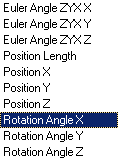
\includegraphics[width=0.25\textwidth]{Figures/7-PositionmatrixOperations}
\end{wrapfigure}

Totally 10 derived quantities may be plotted for a {\sl Position matrix} result
item (as shown to the right). The {\sl Euler Angle} quantities (top three) are
the indicated angles computed from an imagined incremental rotation from the
global coordinate system axes to the orientation represented by the position
matrix. The bottom three items are similar quantities computed from a
Rodriguez parameterization of the incremental rotation.
See the \FedemTGuide{Section 2.3, "Finite Rotation"}
for the definition of these angular quantities.

\subsubsection{Plotting internal control variables}

When you plot internal control variables, you will probably discover that some
of the control lines don't have any results. The reason for this is that more
than one control line share the same control variable, and the results appear
on only one of these (usually the one with the lowest ID).
This situation will occur when one element's output is used as input to more
than one other element.

\Tip{Have the {\rm Control Editor} view open during curve result selection.
  If you select a control line in the RDB selector dialog box, that line will
  also be highlighted in the {\rm Control Editor} view. Vice versa, if you
  select a control line in the {\rm Control Editor} view, that control line
  will be selected in the RDB selector dialog box. That way you can easily see
  which control line you will have to plot to get the variable you want.}

\SubSubSection{Creating curves from file}{creating-curves-from-file}

A curve can be created from an external file by selecting the {\sl From file}
option on the Property Editor panel's {\sl Data} tab. The panel used to define
such a curve is shown below.

\clearpage\noindent
\begin{picture}(343,90)
  \put(0,5){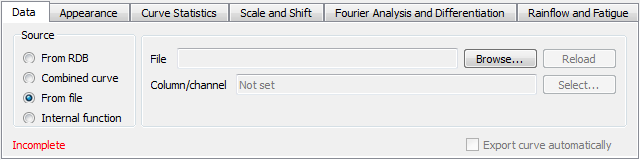
\includegraphics[width=\textwidth]{\ReferenceImg/prp/curve-3}}
  \put(100,55){\Bullet{1}}
  \put(280,55){\Bullet{2}}
  \put(330,55){\Bullet{3}}
  \put(170,40){\Bullet{4}}
  \put(330,40){\Bullet{5}}
\end{picture}

\begin{bulletlist}
\item{\sl File} --
  The selected curve data file will be shown here.

\item\textbf{Browse...} button --
  Opens a dialog box for selection of curve data file.
  The supported file formats are ASCII, nCode DAC and MTS RPC III.

\item\textbf{Reload} button --
  If your data file has changed, you can click this button to reload the curve
  into the viewer.

\item{\sl Column/channel} --
  The name of the selected channel will appear here.
  (Only applicable for multi-column ASCII and MTS RPC III files.)

\item\textbf{Select...} button --
  If you imported a multi-column ASCII file, or a MTS RPC III file,
  you have to select which column or channel to extract data from.
  A dialog box for doing so will appear when clicking this button.
\end{bulletlist}

\vskip\parskip
ASCII curve data files may consist of two or more columns of data.
The columns can be separated by either white-space (one or more tab- or
space-characters) or the comma-character ({\tt,}). The first column is taken
as the $X$-axis values. If more than two columns are present in the file,
the actual column to use for the $Y$-axis values is selected from the
dialog box appearing when clicking the \textbf{Select...} button.
The columns are here identified by numbers (1 up to number of columns minus 1,
the first column of the file is not listed). However, it is also possible to
include user-defined descriptions of the columns.
This is done by inserting as the first line of the file, the string
{\tt\#DESCRIPTION} followed by a tab-separated list of headings for each
column (not for the first column).

\Caution{It is not possible to use comma ({\tt,}) as decimal point in ASCII
  curve data files in Fedem, as this character is interpreted as a column
  separator. Only ({\tt.}) is valid. Therefore, if you have data files exported
  from, e.g., a Norwegian version of Microsoft Office Excel, make sure that the
  decimal point is correct before importing the file into Fedem.}

The nCode DAC and MTS RPC III formats are proprietary binary formats.
DAC support single-columns files only whereas RPC supports multiple columns
(or channels). Please refer to documentation from nCode and MTS for further
details on these formats.

An alternative way of creating curves from file,
is to import multiple curves into an existing or a new graph,
see \refSection{importing-curves-and-graphs}{Importing Curves and Graphs}.

\SubSubSection{Creating curves from a function}{creating-curves-from-a-function}

A curve can be created from one of the functions defined in your model by
selecting the \textbf{Internal function} option on the Property Editor panel's
{\sl Data} tab. The panel used to define such a curve is shown below.

\noindent
\begin{picture}(343,90)
  \put(0,0){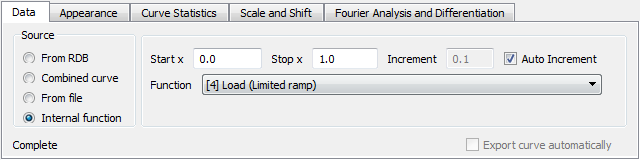
\includegraphics[width=\textwidth]{\ReferenceImg/prp/curve-4}}
  \put(150,60){\Bullet{1}}
  \put(180,35){\Bullet{2}}
  \put(265,55){\Bullet{3}}
\end{picture}

\begin{bulletlist}
\item{\sl Start x}, {\sl Stop x}, {\sl Increment} --
  Sets the end points for the domain to plot,
  and the rate at which the function is sampled.

\item{\sl Function} --
  The function to be plotted is chosen from this pull-down menu.
  The menu lists all functions currently in your Fedem model.

\item{\sl Auto Increment} --
  Most functions have the option to have the resolution set automatically.
  If used, Fedem will determine which points are sufficient to describe the
  function and plot those. In that case the specified increment is not used.
\end{bulletlist}

\Note{If plotting a Poly-line function with {\rm Auto Increment} set, the
  {\rm Start x} and {\rm Stop x} field values are not used either. In this case,
  the $X$-axis domain is automatically adjusted to fit the curve point data.}

\SubSubSection{Creating combined curves}{creating-combined-curves}

A curve can be created as a combination of any of the (up to 10) other curves
currently defined in your model by selecting the {\sl Combined curve}
option on the Property Editor panel's {\sl Data} tab.
The panel used to define such a curve is shown below.

\clearpage\noindent
\begin{picture}(343,95)
  \put(0,5){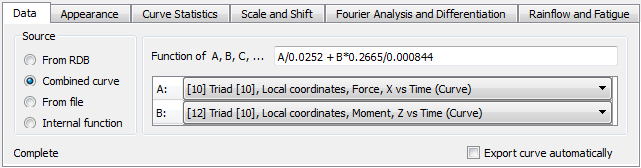
\includegraphics[width=\textwidth]{\ReferenceImg/prp/curve-2}}
  \put(240,60){\Bullet{1}}
  \put(329,35){\Bullet{2}}
\end{picture}

\begin{bulletlist}
\item{\sl Function of A, B, C, ...} --
  In this field you may type in a mathematical expression using the upper case
  letters in range [{\sl A}, {\sl J}] as variables representing other curves in
  the model. Up to 10 other curves may be used in combined curve definition.
  The syntax of the mathematical expression follows that of the Math expression
  function types,
  see \refSubSection{math-expression}{Math Expression}{function-types}.

\item Depending on how many of the variables {\sl A}...{\sl J} you have
  specified in the expression field, a number of pull-down menus labeled
  {\sl A:}, {\sl B:}, etc., are provided here, in which you can assign a curve
  to each variable. Curves of any type may be selected here, also other
  {\sl Combined curves,} except for this curve itself or other combined curves
  referring to this curve either directly or via other combined curves.
\end{bulletlist}

The {\sl Combined curve} feature is an efficient way of plotting result
quantities that are not stored directly in the results database.
For instance, if you want to plot the stress at a certain point in the beam
element you know that this is just a linear combination of the two bending
moments and the axial force at that point along the beam. You can then
set up this linear combination as an expression where the coefficients involved
depends on the cross section geometry, and using the variables {\sl A}, {\sl B}
and {\sl C} to represent the sectional forces involved.
Then you define three other curves plotting these quantities and select select
them in the corresponding pull-down menu in the {\sl Combine curve} properties.

\clearpage


\SubSection{Fourier analysis, differentiation and integration}
           {fourier-analysis-differentiation-and-integration}

Options for performing a Fast Fourier Transform (FFT) of the curve data are
found on the {\sl Fourier Analysis and Differentiation} tab of the Property
Editor panel. The {\sl Fourier Analysis} properties are shown below.

\noindent
\begin{picture}(343,87)
  \put(0,2){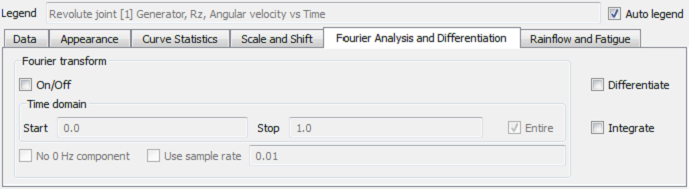
\includegraphics[trim=0 0 0 19,clip,width=\textwidth]{\ReferenceImg/prp/prp-curve-5}}
  \put( 35,50){\Bullet{1}}
  \put( 47,40){\Bullet{2}}
  \put( 15, 4){\Bullet{3}}
  \put(150,13){\Bullet{4}}
  \put(280,49){\Bullet{5}}
  \put(280,28){\Bullet{6}}
\end{picture}

\begin{bulletlist}
\item{\sl Fourier transform, On/Off} --
  When toggled {\sl On} the plotted curve is replaced by its discrete
  Fourier transform (the Fourier transform is a representation of the curve
  in the frequency domain). The value plotted is the magnitude of the transform.

  \EnumNote{The scale and shift parameters specified for the curve
    (see \refSection{scale-and-shift}{Scale and Shift}) are applied to
    the curve data \underline{before} the transform is computed.
    You may \underline{not} scale or shift the transformed curve.}

\item{\sl Time Domain} --
  What part of the curve to transform is specified using these options.
  If {\sl Entire} is toggled {\sl On}, then data for the curve's entire domain
  is used. If {\sl Entire} is toggled {\sl Off}, then a start and stop time
  may be set in the fields labeled {\sl Start} and {\sl Stop}, repsectively.

\item{\sl No 0 Hz component} --
  The arithmetic mean of the original curve data is reflected in the transform's
  value at 0 Hz (the transform's first point). To facilitate transform analysis
  you might want to cancel out the 0 Hz component by using this option.

\item{\sl Use sample rate} --
  The sample rate used in the transform is by default equal to that of the curve
  data. However, if the curve has a non-constant sample rate the transform will
  fail. In such cases the wanted sample rate may be input using this field.

\item{\sl Differentiate} --
  When this toggle is enabled, the plotted curve is replaced by its derivative,
  which is computed from the curve point values $f_i=f(x_i)$ through the formula
  $$
    f'(x_i) = \frac{1}{2}\left( \frac{f_{i+1}-f_{i}}{x_{i+1}-x_{i}} +
                                \frac{f_{i}-f_{i-1}}{x_{i}-x_{i-1}} \right)
  $$

\item{\sl Integrate} --
  When this toggle is enabled, the plotted curve is replaced by the integral of
  the curve data, which is computed from the curve point values through the
  recursive formula
  $$
    \int\limits_{x_0}^{x_i}f(x)dx =
    \int\limits_{x_0}^{x_{i-1}}f(x)dx + \frac{1}{2}(f_i+f_{i-1})(x_i-x_{i-1})
  $$
\end{bulletlist}

\Caution{The Fourier transform needs to be recalculated
  each time points are added to the curve.
  Consequently, if curves are plotted while the Dynamics solver is run,
  then transforming these curves will increase the CPU load during solving.}

\Tip{A good reference on the theory of Fourier transforms is:
  W. Rudin, "Real and Complex analysis", McGraw-Hill, 1974.}


\SubSection{Scale and Shift}{scale-and-shift}

Options to scale and shift the curve data are found on the {\sl Scale and Shift}
tab of the Property Editor panel. You may apply scaling and a shift on the curve
data independently in the $X$- and $Y$-directions.
The {\sl Scale and Shift} properties are shown below.

\noindent
\begin{picture}(343,85)
  \put(0,0){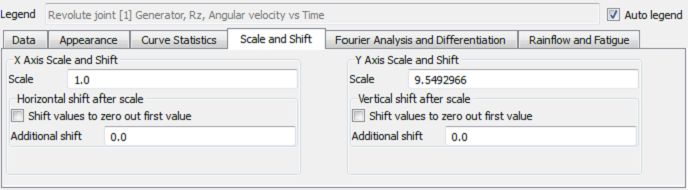
\includegraphics[trim=0 0 0 19,clip,width=\textwidth]{\ReferenceImg/prp/prp-curve-4}}
  \put(-11,50){\Bullet{1}}
  \put(160,50){\Bullet{1}}
  \put(-10,32){\Bullet{2}}
  \put(162,32){\Bullet{2}}
  \put(-10,21){\Bullet{3}}
  \put(162,21){\Bullet{3}}
\end{picture}

\begin{bulletlist}
\item{\sl Scale} --
  Scale factor applied to the $X$- or $Y$-axis values.

\item{\sl Shift values to zero out first value} --
  For the $X$-axis; shift the curve horizontally such that its first $X$-value
  becomes zero.
  For the $Y$-axis; shift the curve vertically such that its first $Y$-value
  becomes zero.

\item{\sl Additional shift} --
  Additional horizontal/vertical shift (i.e., in addition to the zero-out
  operation, if applied) in the curve's $X$/$Y$-values.
\end{bulletlist}

\Note{Scaling the $Y$-axis of a curve will affect the results of fatigue
  and damage calculations (see \refSection{fatigue-calculation}
  {Fatigue calculation from standard S-N curves}).}


\SubSection{Appearance}{appearance}

The Curve appearance can be altered by selecting the {\sl Appearance} tab
in the Property Editor panel. The associated properties are shown below.

\noindent
\begin{picture}(344,80)
  \put(0,0){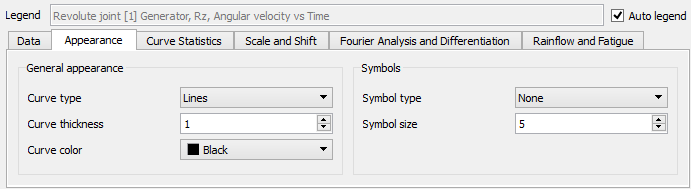
\includegraphics[trim=0 0 0 27,clip,width=\textwidth]{\ReferenceImg/prp/prp-curve-2}}
  \put( 75,41){\Bullet{1}}
  \put( 75,28){\Bullet{2}}
  \put( 75,16){\Bullet{3}}
  \put(240,41){\Bullet{4}}
  \put(240,28){\Bullet{5}}
\end{picture}

\begin{bulletlist}
\item{\sl Curve Type} --
  You can select {\sl Lines}, {\sl Dots}, or {\sl Invisible} from the
  {\sl Curve Type} pull-down menu.

\item{\sl Curve thickness} --
  You can adjust the curve thickness with 5 different levels,
  from 0 (thinnest) to 4 (thickest).

\item{\sl Curve Color} --
  Use the drop-down menu to select a different curve color.
  You may either select one of the pre-defined colors, or create a new by
  selecting {\sl More...} at the bottom of the drop-down menu.

\item{\sl Symbol type} --
  You can select a symbol (cross, circle, triangle, etc.) to display on the
  curve. A symbol will be shown on all points of the curve,
  so use this with care if it consists of a huge number of points.

\item{\sl Symbol Size} --
  Use the spin box to control the size of the symbols.
\end{bulletlist}


\SubSection{Curve Statistics}{curve-statistics}

On the {\sl Curve Statistics} tab you can display different statistical
properties of a curve. The associated properties are shown below.

\noindent
\begin{picture}(343,85)
  \put(0,0){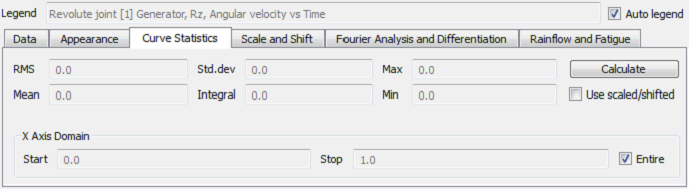
\includegraphics[trim=0 0 0 19,clip,width=\textwidth]{\ReferenceImg/prp/prp-curve-3}}
  \put(56,54){\Bullet{1}}
  \put(56,41){\Bullet{2}}
  \put(150,54){\Bullet{3}}
  \put(150,41){\Bullet{4}}
  \put(230,54){\Bullet{5}}
  \put(230,41){\Bullet{6}}
  \put(323,55){\Bullet{7}}
  \put(286,32){\Bullet{8}}
  \put(50,22){\Bullet{9}}
\end{picture}

\begin{bulletlist}
\item{\sl RMS} --
  The Root Mean Square value, found from
  $$
    y_{rms} = \sqrt{\frac{1}{n}\sum_{i=1}^n y_i^2}
  $$

\item{\sl Mean} --
  The Mean value, $\bar{y}=\frac{1}{n}\sum_{i=1}^n y_i$.

\item{\sl Std.dev.} --
  The Standard Deviation (biased), found from:
  $$
    \sigma = \sqrt{\frac{1}{n}\sum_{i=1}^n ({y_i}-{\bar{y}})^2}
  $$

\item{\sl Integral} --
  By the Trapezoid rule.

\item{\sl Max} --
  The overall maximum of the $y$-values in the curve data set.

\item{\sl Min} --
  The overall minimum of the $y$-values in the curve data set.

\item\textbf{Calculate...} --
  Press this button to retrieve the statistical values.

\item\textbf{Use scaled/shifted} --
  Toggling on this button will make the calculation take into account any scale
  and shift values defined in the {\sl Scale and Shift} tab
  (see \refSection{scale-and-shift}{Scale and Shift}), and in effect
  do the calculations on the curve as it is shown in the graph view.
  If the button is toggled off, the unprocessed data will be used.

\item{\sl X Axis Domain} --
  Toggle the \textbf{Entire} button on to use all the data points on the curve,
  or specify a start and a stop value. If you specify an interval,
  two vertical lines at the start and stop values, will appear in the graph view
  when you click the \textbf{Calculate...} button.
\end{bulletlist}


\SubSection{Fatigue calculation from standard S-N curves}{fatigue-calculation}

Options to assess fatigue results based on plotted stress histories are found
in the {\sl Rainflow and Fatigue} tab of the Property Editor panel.
The associated properties are shown below. Here, you may select different
standard S-N curves to base the damage calculation on, specify a time interval
for the damage calculation, and evaluate the equivalent life in days, hours or
repeats. For details on how the damage is calculated from a given time history
response, see the \FedemVer~Theory Guide.

\noindent
\begin{picture}(130,85)
  \put(0,0){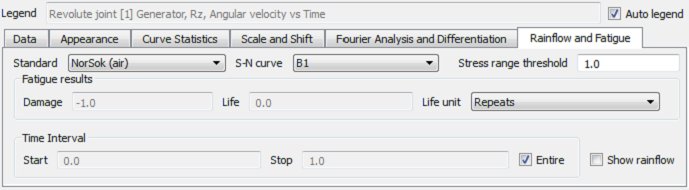
\includegraphics[trim=0 0 0 18,clip,width=\textwidth]{\ReferenceImg/prp/prp-curve-6}}
  \put( 80,59){\Bullet{1}}
  \put(170,59){\Bullet{2}}
  \put(310,59){\Bullet{3}}
  \put( -3,39){\Bullet{4}}
  \put( -3,10){\Bullet{5}}
  \put(295,20){\Bullet{6}}
\end{picture}

\begin{bulletlist}
\item{\sl Standard} --
  Select the fatigue standard to use in the calculation.

\item{\sl S-N curve} --
  Select an S-N curve from the selected standard.

\EnumTip{The S-N curve standards listed in the Fatigue tab are defined in the
  file \File{sn\_curves.fsn} located in the installation directory of Fedem.
  The syntax of the S-N curve definitions is description in the header of this
  file, and it is possible to add your own S-N curve definitions to it also.}

\item{\sl Stress range threshold} --
  Stress ranges with magnitude below this threshold are ignored in the stress
  cycle counting (rainflow analysis).

\item{\sl Damage}, {\sl Life}, {\sl Life unit} --
  The {\sl Fatigeu Results} frame displays the damage results for the plotted
  stress history. The life is displayed in days, hours or repeats,
  depending what you select from the {\sl Life unit} drop-down.

\item{\sl Start}, {\sl Stop}, {\sl Entire} --
  You can specify what part of the curve to use for fatigue calculations by
  setting the {\sl Time Interval} options. If {\sl Entire} is toggled {\sl On},
  data for the entire domain of the curve is used. If it is toggled {\sl Off},
  the time interval is specified by the {\sl Start} and {\sl Stop} fields.

\item{\sl Show rainflow} --
  When this toggle is enabled, the plotted curve is replaced by the results of
  the Rainflow calculation, i.e., it shows the magnitudes of the stress ranges
  that are the basis of the subsequent damage calculation.
\end{bulletlist}

\Note{If the $Y$-axis of the curve is scaled,
  the scaling factor will be applied to the damage calculations too
  (see \refSection{scale-and-shift}{Scale and Shift}).}


\subsection{View control}

In graph views, you can manipulate the display using the \textbf{Zoom and Pan}
tool bar shown below. For the use of these commands,
see \refSection{zoom-and-pan}{Zoom and Pan}.

\vskip\parskip
\begin{center}
  
\includegraphics[width=0.6\textwidth]{Figures/zoom-pan-toolbar}
\end{center}

You can also use the Dynamic Pan 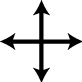
\includegraphics[scale=0.7]{Figures/pan}
(\textbf{F1}) and Dynamic Zoom 
\includegraphics[scale=0.7]{Figures/zoom}
(\textbf{F2}) commands, in the same way as they are used in the {\sl Modeler}
view (see \refSection{navigation}{3D Navigation}).

The following can be useful tips when viewing graphs:

\begin{itemize}\item
  If the number of points in your graph is very high, dynamic panning and
  zooming can take a long time; use the commands on the \textbf{Zoom and Pan}
  tool bar instead to speed up graphic performance.
\end{itemize}

\clearpage
\IconText{zoomWindow}{\vskip-5mm
  \begin{itemize}\item
    You can use the \textbf{Zoom Window} command to zoom in on a small area,
    enabling you to see the curves in that area with greater detail. This
    command is turned on if the \textbf{Z} key is pressed while viewing a graph.
  \end{itemize}}

\vskip-3mm
\IconText{zoomWindowAutoscale}{\vskip-5mm
  \begin{itemize}\item
    You can use the \textbf{Zoom Window With Autoscale} command to zoom in on
    an area. The contents inside the zoom rectangle will be scaled to fit
    inside the graph view. This command is turned on whenever the
    \textbf{X} key is pressed while viewing a graph.
  \end{itemize}}

\vskip-3mm
\IconText{zoomAll}{\vskip-5mm
  \begin{itemize}\item
    To adjust the graph axes so that the entire curves fit into the graph view,
    click the \textbf{Zoom All} button, or press \textbf{F5}.
  \end{itemize}}


\SubSection{Export of Curve data}{export-of-curve-data}

Curve and Graph objects in Fedem can be exported to files
for further processing in external software.
We distinguish between exporting graphs and exporting curves.

\subsubsection{Curve export}

When exporting one or more curves, each curve is written to a separate file.
The file format can be either Single Column ASCII, nCode DAC or MTS RPC III
time history file.

\begin{wrapfigure}[13]{r}{0.5\textwidth}
  \vspace{-5mm}
  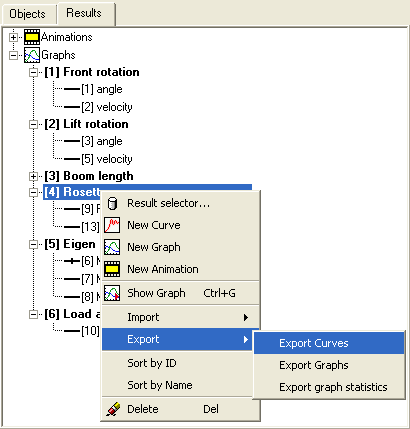
\includegraphics[width=0.46\textwidth]{Figures/7-CurveExport}
\end{wrapfigure}

To export curves, select the curve or curves you want to export in
the Model Manager {\sl Results} list, right-click and select
\textbf{Export} $\rightarrow$ \textbf{Export Curves...}
A dialog box will then pop up. If you have selected only one curve,
you can select location and file name of the exported curve.
If you have selected several curves, you must select a directory to export to.
If you select a graph, all its curves will be exported.

\medskip
When you select a directory to export to, the files will be given
names automatically. The file name will be on the form:

{\tt G\_\textless OwnerGraphID\textgreater\_C\_\textless CurveID\textgreater\_\textless CurveDescription\textgreater.\textless Format\textgreater}

\Tip{Curves that plot result data from the Dynamics Solver may also be exported
  automatically when the solver has finished
  (see \refSubSection{output-tab}{Output tab}{dynamics-solver-advanced-mode}).}

\Note{The exported data is equal to the results from the settings in the
  Fourier Analysis tab and the Scale and Shift tab. If you want to export
  unprocessed data, go to these tabs and set all the values back to default (see
  \refSection{fourier-analysis-differentiation-and-integration}
             {Fourier analysis, differentiation and integration} and
  \refSection{scale-and-shift}{Scale and Shift}).}

\Caution{When exporting to nCode DAC or MTS RPCIII,
  $\Delta x$ needs to be constant across the entire data set.
  Using either Physical Time with constant time step size,
  or Time Step Number will satisfy this requirement.}

\subsubsection{Graph export}

\begin{wrapfigure}[12]{r}{0.47\textwidth}
  \vspace{-10mm}
  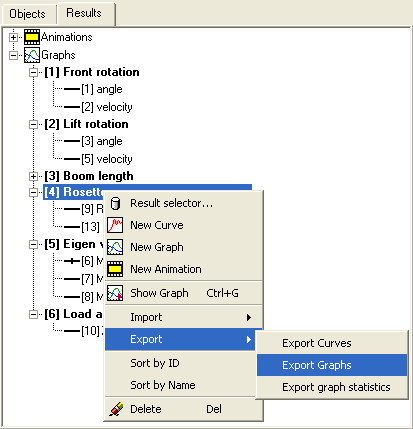
\includegraphics[width=0.45\textwidth]{Figures/7-GraphExport}
\end{wrapfigure}

When exporting one or more graphs, each file exported will contain several
curves. The file format is either Multi Column ASCII or MTS RPC III
time history file.

Select the graph or graphs you want to export in the Model Manager
{\sl Results} list, right-click and select \textbf{Export} $\rightarrow$
\textbf{Export Graphs...} A dialog box will then pop up, with slightly
different appearance depending on what you have selected.

If you have selected one graph, or a collection of curves belonging to the same
graph, the dialog box will let you select directory, file name and format for
the exported graph file. If you selected only a subset of curves from a graph,
only the selected curves will be written to the graph file.

If you have selected several graphs and/or curves belonging to different
graphs, the dialog box will let you specify a directory to write the
files to and the file format. One file is the written to the specified
directory for each selected graph. The name of each file is assigned
automatically, and will be on the form
{\tt G\_\textless GraphID\textgreater\_\textless GraphDescription\textgreater.\textless Format\textgreater}.

\Caution{When exporting graphs, all curves in the selection must have equal
  $x$-axis definitions, both in terms of number of data points and
  increment $\Delta x$. When exporting to Multi-Column ASCII, the $X$-axis
  values of the exported graph are thus set identical to those of the
  first curve in the selection. Subsequent curves having a lower
  resolution in their data sets will then be interpolated, where needed;
  if they have a higher resolution, some data points will be omitted in
  the exported graph. When exporting to MTS RPC III, the constant
  increment $\Delta x$ for the graph is selected as the smallest increment
  between two data points among all the selected curves. Curves having a lower
  resolution than this increment will then be interpolated, where needed.}

\Tip{To export a single curve or graph, you may also use the \textbf{Export}
  and \textbf{Export Object...} item in the \textbf{File} menu,
  after selecting the desired curve or graph.}


\SubSection{Importing Curves and Graphs}{importing-curves-and-graphs}

Curve data can be imported into Fedem both as single curves,
and complete graphs.

\subsubsection{Importing Curves}

\begin{wrapfigure}[11]{r}{0.5\textwidth}
  \vspace{-10mm}
  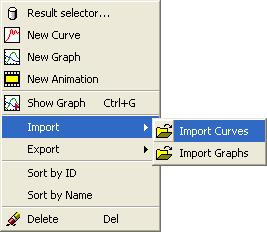
\includegraphics[width=0.48\textwidth]{Figures/7-CurveImport}
\end{wrapfigure}

To start importing curves, right-click with your mouse on a graph, a curve
or on an empty spot in the Model Manager {\sl Results} list and select
\textbf{Import} and \textbf{Import Curves}. In the dialog box that pops
up, select one or more files you want to import. One curve is created
for each file. For details on the supported file formats, see
\refSubSection{creating-curves-from-file}{Creating curves from file}
              {curve-properties}.

If you right-clicked on a a graph, the curve data will be imported into
that graph, whereas if you clicked on a curve, the data will be imported
into the graph containing that curve. If you clicked on an empty spot, a
new graph will be created for the new curve(s).

\subsubsection{Importing Graphs}

To start importing graphs, right-click with your mouse anywhere in the
Model Manager {\sl Results} List and select \textbf{Import} and
\textbf{Import Graphs}. In the dialog box that pops up, select one or more graph
files you want to import. One graph is created for each of the selected files,
containing one curve for every column or channel in the file.


\subsection{Exporting to picture files}

You may also want to export a graph view to a picture file.
This is accomplished by first selecting the {\sl Graph} view you want to export
and then selecting \textbf{Export} and \textbf{Export View...} from the
\textbf{File} menu. You may choose to output in either BMP, JPEG or PNG file
format. See \refSection{exporting-a-part}{Exporting a part},
for more about the export capabilities in Fedem.


%Feature removed long ago..
%\subsection{Printing graphs}
%When a {\sl Graph} view is active, you can send its contents directly to a
%printer for printing. Select the printer symbol on the tool bar, or the
%\textbf{Print With Setup} command in the \textbf{File} menu. When selecting the
%latter, you will be able to select which printer to use, paper format and so on.


%%%%%%%%%%%%%%%%%%%%%%%%%%%%%%%%%%%%%%%%%%%%%%%%%%%%%%%%%%%%%%%%%%%%%%%%%%%%%%%%
\Section{Beam diagrams}{beam-diagrams}

In addition to viewing the evolution of a result quantity at a fixed point in
the model as a function of time (or any other fixed simulation quantity),
as described above, it is often desirable to view the variation of a quantity
along a one-dimensional structure, such as a beamstring, at a given time.
For this purpose, we offer the possibility to create {\sl Beam diagram} graphs.


\subsection{Creating beam diagrams}

\IconTextFirst{createGraph}{
  The only way to create a beam diagram graph is to select
  \textbf{New Beam diagram} from the \textbf{Result} menu,
  or right-click in the Model Manager {\sl Results} list and select
  \textbf{New Beam diagram}.
  There is no drag-and-drop creation option here, as for the regular graphs.
  The created graph titled "New Graph" is then listed in the
  {\sl Results} list of the Model Manager panel.}

\IconText{createCurve}{
  To create curves in a beam diagram graph, select the graph to which you want
  to add the curve and select \textbf{New Curve} from the \textbf{Result} menu
  or the right-click menu in the Model Manager {\sl Results} list.
  The created curve titled "New Curve" is then listed under the selected
  beam diagram graph.}

The description and other properties of the beam diagrams and their curves may
be edited in the same way as for other graphs and curves.

\clearpage
\begin{wrapfigure}[8]{r}{0.5\textwidth}
  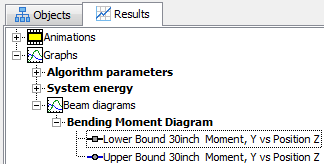
\includegraphics[width=0.5\textwidth]{Figures/7-BeamDiagram}
\end{wrapfigure}

All beam diagram graphs are grouped under the tree-node labeled
{\sl Beam diagrams} in the {\sl Results} list (shown to the right).
This is to make the distinction of these type of curves compared to all the
other curve types more clear. It is not possible (and makes no sense either)
to mix these types of curves with the other curves within the same graph.
A curve in a beam diagram can only be copied or moved into an other beam
diagram graph, and not into the other graphs. Similarly, a regular curve
can not be copied or moved into a beam diagram graph.


\subsection{Beam diagram curve properties}

The properties of a beam diagram graph are identical to those of the regular
graphs (see \refSection{graph-properties}{Graph properties}), except for that
the {\sl Start time} and {\sl Stop time} fields and the {\sl Use time interval}
toggle are absent.

The curves in a beam diagram has a slightly different Property Editor panel,
compared with the other curves. The {\sl Data} tab reflects the nature of this
curve type and is shown below The other three tabs ({\sl Appearance},
{\sl Curve Statistics} and {\sl Scale and Shift}) are similar as for the regular
curves (see \refSection{curve-properties}{Curve properties}) whereas the
{\sl Fourier Analysis and Differentiation} tab and the
{\sl Rainflow and Fatigue} tab both are absent.

\noindent
\begin{picture}(343,115)
  \put(0,0){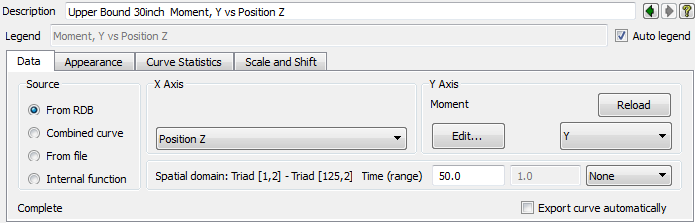
\includegraphics[width=\textwidth]{Figures/7-SpatialCurveProperty}}
  \put( 30,63){\Bullet{1}}
  \put( 63,18){\Bullet{2}}
  \put( 95,63){\Bullet{3}}
  \put(230,63){\Bullet{4}}
  \put(330,37){\Bullet{5}}
  \put(265,17){\Bullet{6}}
  \put(330,18){\Bullet{7}}
  \put(330,53){\Bullet{8}}
\end{picture}

\begin{bulletlist}
\item{\sl Source} --
  The same choices are available here as for regular curves.
  However, for {\sl Combined curves}, only other beam diagram curves having
  identical $X$-axis definitions may be selected in their definition.

\item{\sl Spatial domain} --
  This shows the selected range of objects (Triads or Beams)
  from which the results plotted by the curve are extracted.

\item{\sl X Axis} --
  Defines the coordinate value used for the $X$-axis definitions.
  The choices are {\sl Position X}, {\sl Position Y}, {\sl Position Z} and
  {\sl Length}. The first three choices indicate the corresponding global
  position coordinate of the Spatial domain objects, whereas {\sl Length}
  is a running coordinate along the spatial objects.
  The latter is useful when the beamstring is curved or not parallel to
  one of the global coordinate axes.

\item{\sl Y Axis} --
  Defines the result quantity to be plotted.
  Click the \textbf{Edit...} button to open the RDB selector dialog box
  where you can pick the wanted result (see
  \protect\hyperlink{selecting-rdb-results}{\sl"Selecting RDB results"}
  below for details). Alternatively, you may also right-click the curve in the
  Model Manager {\sl Results} list and then select \textbf{Edit Y Axis...}

\item{\sl Result Operation} --
  The pull-down menu next to the \textbf{Edit...} button lists mathematical
  operations (such as extracting the $X$-component or computing the length of a
  vector) related to the selected result quantity. The content of this menu
  depends on the chosen result quantity, in the same way as for the regular
  curves.

\item{\sl Time (range)} --
  These fields specify the time or the time range at which the plotted results
  should be extracted.

\item{\sl Time operation} --
  This pull-down menu specifies the mathematical operation that is applied to
  the result quantity over the selected time range, in order to compute the
  value to be plotted. The default choice {\sl None} just extracts the results
  at the time specified in the first of the two {\sl Time (range)} fields.
  The other options available are {\sl Min}, {\sl Max}, {\sl Abs Max},
  {\sl Mean} and {\sl RMS} (root-mean-square).

\item\textbf{Reload} --
  This button activates a manual reload of the data to be plotted.
  If you are viewing a beam diagram graph while the dynamics solver is running
  you need to click on this button to update the plot when new results are
  available. Unlike the regular curves plotting time histories,
  beam diagram curves are not updated automatically.
\end{bulletlist}

\subsubsection{Selecting RDB results}

To select the results to plot in a beam diagram curve,do the following steps:

\begin{enumerate}
\item
  In the {\sl Results} list of the Model Manager panel, select the Beam diagram
  curve that you want to edit. Its properties are displayed in the Property
  Editor panel.
\item
  In the Property Editor panel, click the \textbf{Edit...} button for the
  $Y$-axis, or right-click on a curve in the Model Manager {\sl Results} list
  and select \textbf{Edit Y Axis...} The RDB selector dialog box (see
  \refSubSection{selecting-rdb-results}{Selecting RDB results}
                {curve-properties}) is then opened.
\item
  Select a mechanism object from the {\sl Existing Results} list or the
  {\sl Modeler} view that represent the starting point of the beam diagram
  curve. Only {\sl Triad} and {\sl Beam} elements may be selected.
  Selection of any other object is ignored.

  \EnumNote{If the mechanism analysis have been performed, variables for
    the selected object are listed in the {\rm Existing Results} list.
    If you have not yet performed an analysis, variables are listed in the
    {\rm Possible Results} list instead.}
\item
  Select a variable to be used as the $Y$-coordinates from either the
  {\sl Existing Results} or {\sl Possible Results} lists, and click \textbf{OK}
  to close the panel or \textbf{Apply} to continue variable selection.
\end{enumerate}

The {\sl Triad} or {\sl Beam} that you select in Step 3 above needs to be at the
end of a beam string, i.e., the Triad can only be attached to one Beam object,
or the Beam (if selected) can only have a neighboring Beam in one of its ends.
If these conditions are not fulfilled, the selection is rejected and the curve
does not appear in the graph view.

When a valid object selection has been made, the beam topology is traversed
automatically to determine the {\sl Spatial domain} objects
(see bullet 2 above). The traversal is continued until the opposite end of the
beam string, or until a Triad connected to three or more Beams is encountered.

\Note{If a beam string is connected to another (but only one) beam string via a
  single-master joint (Rigid, Revolute, Ball or Free joint), the beam diagram is
  continued across that joint. When plotting such beam diagram curves, you may
  see discontinuities in the plot reflecting the location of that joint.}

\Caution{Using {\rm Length} as the $X$-axis definition (see bullet 3 above)
  is not recommended if the beam string is interrupted by a joint, because the
  length coordinate (which is calculated based on updated coordinate values)
  will then start from zero again on the other side of the joint.
  It is then better to select the {\rm Position X, Y} or {\rm Z} value
  that best corresponds to the axis direction of the beamstring.}

\clearpage


%%%%%%%%%%%%%%%%%%%%%%%%%%%%%%%%%%%%%%%%%%%%%%%%%%%%%%%%%%%%%%%%%%%%%%%%%%%%%%%%
\Section{Graph groups}{graph-groups}

In a similar way as sub-assemblies can be used to group mechanism objects
(see \refSection{sub-assemblies}{Sub-assemblies}), {\sl Graph groups} can be
created to organize the graphs of a complex model into logic units.

\IconText{graphGroup}{
  To create a new graph group object, select \textbf{New Graph group}
  from the \textbf{Result} menu, or right-click anywhere in the Model Manager
  {\sl Results} list and select \textbf{New Graph group}.}

\begin{wrapfigure}[8]{r}{0.35\textwidth}
  \vspace{-5mm}
  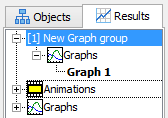
\includegraphics[width=0.35\textwidth]{Figures/7-GraphGroup}
\end{wrapfigure}

A new Graph group containing one empty Graph then appears in the {\sl Results}
list of the Model Manager panel (shown at right).

More graphs can be added to the graph group by keeping it selected
(highlighted) while creating new Graphs. It is also possible to
drag-and-drop result items from the RDB selector dialog box onto a Graph
group to create a new graph there with a curve plotting that item. (See
\protect\hyperlink{graph}{\sl"Graph"} and
\refSubSection{creating-curves-and-graphs-by-drag-and-drop}
              {Creating curves and graphs by drag and drop}
              {creating-graphs-and-curves}.

\Note{Only graphs with curves plotting time history results can be organized in
  graph groups, i.e, Beam diagrams can not be created in a graph group object.
  One may instead say that Beam diagrams constitute a graph group by itself.}

A graph group is in many ways equivalent to a sub-assembly for
mechanism objects, except that it does not contain any positioning data.
The Property Editor panel for graph groups thus only contains the
{\sl Subassembly model file} field (see below), through which the graph
groups can be assigned a file name such that it can be re-used in
another model with a similar graph setup.

\noindent
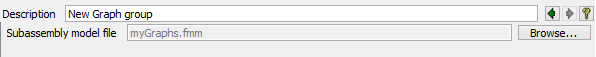
\includegraphics[width=\textwidth]{Figures/7-GraphGroupProperty}

See \refSection{sub-assembly-properties}{Sub-assembly properties}
for details on how the Subassembly model file field is used.

\clearpage


%%%%%%%%%%%%%%%%%%%%%%%%%%%%%%%%%%%%%%%%%%%%%%%%%%%%%%%%%%%%%%%%%%%%%%%%%%%%%%%%
\Section{Animations}{animations}

Fedem animations are used to visualize the motion or the structural results of
your model in an intuitive and life-like fashion. Fedem is able to
utilize part motion, part deformation and
part color contours to visualize
your results and help you understand them.

\begin{center}
  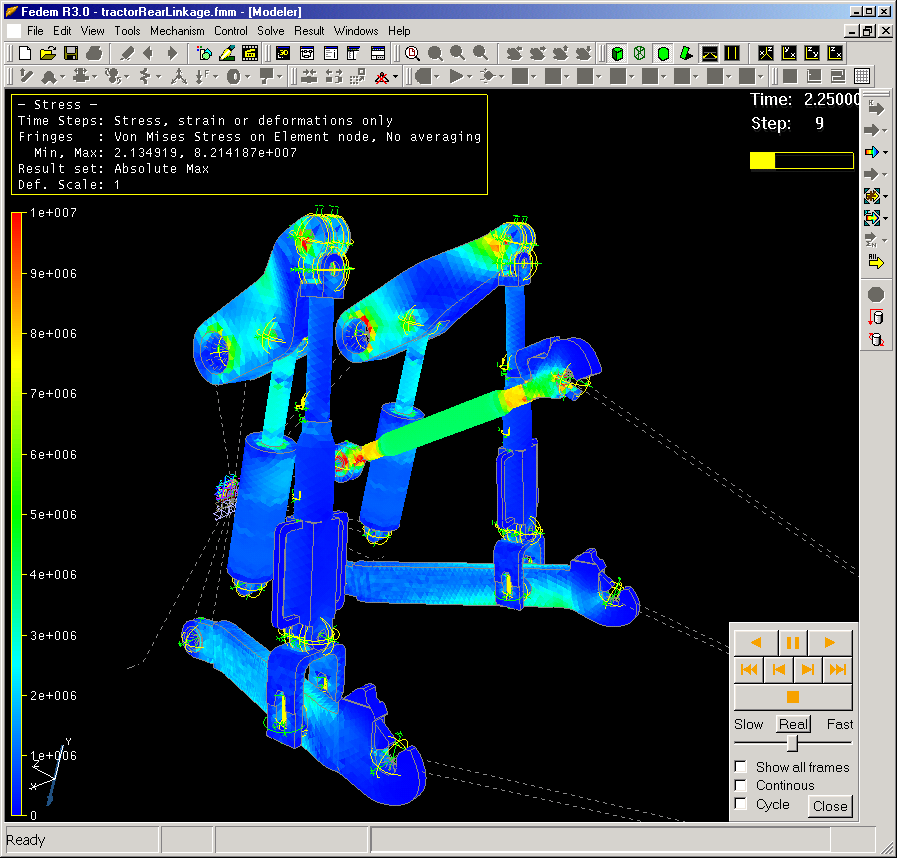
\includegraphics[width=0.9\textwidth]{Figures/AnimationStresstractorRearLinkage}
\end{center}

You can create several Animation objects and define different options for each
animation. The created animations can then be loaded into the {\sl Modeler}
view one at a time.

Animation objects can be set up before or after performing the dynamics
simulation and other analyses. If you create a certain type of animation and
load it into the {\sl Modeler} view before starting the simulation, you can
observe the mechanism motion during the simulation as it is constantly updated
(see \refSection{interaction-during-processing}{Interaction during processing}).
Otherwise, you can view the entire animation after the simulation is complete.

When an animation is loaded it can be controlled using the Play panel
(see \refSection{play-panel}{Play panel}) and the Animation Control dialog box
(see \refSection{animation-controls}{Animation controls}).
The Play panel is displayed in the lower right corner of the {\sl Modeler} view
(as shown above) when loaded.
The Animation Control dialog box can be activated when needed.
Graphs plotting values vs.\ time will also be animated in the sense that
a bar showing the time of the current animation frame is shown.
This time bar is present only as long as the animation is showing a time step.

\Note{You can set up animations at any time and load them.
  However, nothing will appear unless the appropriate results are present.}


\SubSection{Managing animations}{managing-animations}

\subsubsection{Creating animations}

You can create as many animations as you like. It is recommended that you
provide descriptive names for your animations (Stress, Strain, or Eigenmodes,
and so on) as the description is used in the Model Manager {\sl Results} list
to distinguish between the animations.

\IconText{animation}{
  To create an animation, select \textbf{New Animation} on the {\sl Result}
  menu or right-click in the Model Manager {\sl Results} list and select
  \textbf{New Animation} on the shortcut menu.}

\SubSubSection{Loading animations}{loading-animations}

Once the animation is created, you can show it in the {\sl Modeler} view by
performing the following steps:

\vskip\parskip
\IconText{modeler}{\vskip-5mm
  \begin{enumerate}
    \setlength\itemsep{1mm}
  \item
    To open the {\sl Modeler} view, click the \textbf{Show Modeler} button
    on the \textbf{Windows} tool bar (or from the \textbf{Windows} menu).
    The {\sl Modeler} view opens in the Workspace area.
  \item
    Select the animation in the Model Manager {\sl Results} list.
  \item
    Click the \textbf{Load Animation} button in the Property Editor panel,
    or right-click the animation in the {\sl Results} list and select
    \textbf{Load Animation} on the shortcut menu.
  \end{enumerate}}

\vskip-18mm
\IconText{loadAnimation}{\vskip13mm
  The animation is loaded and both
  the Contour Legend and Play Panel are displayed in
  the {\sl Modeler} view (see \refSection{play-panel}{Play panel}).}

\Tip{Changes to animations cannot be updated instantaneously. However,
  after each change you can reload the animation to include the updates.}

\begin{wrapfigure}[6]{r}{0.35\textwidth}
  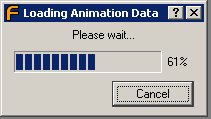
\includegraphics[width=0.35\textwidth]{Figures/7-CancelAnimationLoading}
\end{wrapfigure}

Loading an animation with contours and/or deformations for large FE models may
take a considerable amount of time. However, it is possible to cancel the
animation loading process at any time, by using the \textbf{Cancel} button of
the progress dialog box that appears while the animation is loading
(shown to the right).

\subsubsection{Closing animations}

\IconTextFirst{endAnimation}{
  You can end an animation session at any time by clicking \textbf{Close}
  on the Play Panel or selecting \textbf{End Animation Session}
  from the {\sl Result} menu.}


\SubSection{Animation properties}{animation-properties}

To display the properties of an animation in the Property Editor panel, select
the animation in the Model Manager {\sl Results} list. The properties for the
animation are displayed in the Property Editor panel as shown below.

\noindent
\begin{picture}(343,110)
  \put(0,10){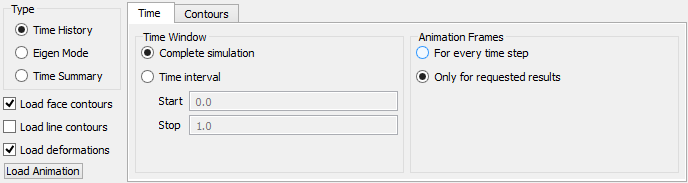
\includegraphics[width=\textwidth]{\ReferenceImg/prp/animation-1}}
  \put( 20,93){\Bullet{1}}
  \put( 57,45){\Bullet{2}}
  \put( 55,33){\Bullet{3}}
  \put( 55,21){\Bullet{4}}
  \put( 45,11){\Bullet{5}}
  \put( 78,93){\Bullet{6}}
  \put(109,93){\Bullet{7}}
\end{picture}

\begin{bulletlist}
\item{\sl Type} --
  The animation type determines the main type of results you want to animate.
  See \protect\hyperlink{animation-types}{\sl"Animation types"} below.

\item{\sl Load face contours} --
  If enabled, the values specified on the Contours tab are loaded and shown as
  color contours on the element faces of the mechanism assembly. See also
  \protect\hyperlink{contours-tab}{\sl"Contours tab"} below.

\item{\sl Load line contours} --
  This option controls whether or not contours are loaded and displayed
  on the FE-mesh lines. The values displayed will be the result selected on the
  Contours tab but always averaged on the nodes. See also
  \protect\hyperlink{contours-tab}{\sl"Contours tab"} below.

  \EnumNote{Element-to-node averaging is not yet supported, and even if
    {\rm Load line contours} is toggled, no contour colors will be shown on the
    mesh lines when the chosen {\rm Result class} is {\rm Element}.}

\item{\sl Load deformations} --
  If enabled, deformation results from the stress or mode shape recovery---
  depending on the animation type selected--- are loaded,
  if such results are present. See
  \refSection{stress-recovery-analysis}{Stress recovery analysis} and
  \refSection{mode-shape-recovery-analysis}{Mode shape recovery analysis}.

\item\textbf{Load Animation} --
  If you make changes to the animation properties, you can reload the animation
  at any time by clicking this button.

\item{\sl Time} tab --
  Options to control what part of the time history to load.
  See \protect\hyperlink{time-tab-animation}{\sl"Time tab"} below.

\item{\sl Contours} tab --
  Options to control what result values to load and display as color contours.
  See \protect\hyperlink{contours-tab}{\sl"Contours tab"} below.
\end{bulletlist}

\SubSubSection{Animation types}{animation-types}

The following three animation types are available.

\begin{enumerate}
\item{\sl Time History} --
  This animation type is used to animate time history results.
  This can be the rigid body component of part motion calculated in the dynamics
  solver, or recovered stress, strain and deformational part of the part motion.

\item{\sl Eigen Mode} --
  This animation type is used to visualize the shape of a system eigenmode at
  a specific point in time. To provide this visual interpretation, the mode
  shape is used to create an animation of the mechanism oscillating as if the
  eigenmode was excited.

  The time displayed along with the progress bar shown during an eigenmode
  animation is the time elapsed during the oscillating motion. The legend text
  displays the point in time for existence of the animated eigenmode during the
  dynamics solution.

  Unless a mode shape recovery has been run, you can only animate the rigid body
  component of the eigenmode for each part. Note that the partitioning of the
  total mode shape into a rigid body approximation plus a deformable component
  depends on the chosen computational coordinate system of the part
  (see the \FedemTGuide{Section 4.1}).
  In particular, if the center of rotation for a mode is far from the origin of
  the part coordinate system, the deformable component may be misleading.
  However, the sum of the deformable and rigid body components will always be
  correct.

\item{\sl Time Summary} --
  These animations are used to show accumulated structural results within
  a specified time interval. These results are produced by running the Strain
  Coat Recovery Summary, e.g., maximal principal stresses reached within a
  the time interval.

  Usually only one frame with accumulated results from the complete simulation
  time are produced and displayed. It is, however, also possible to show an
  animation of how the results are accumulated by running the Strain Coat
  Recovery Summary several times with different stop times.
\end{enumerate}

\SubSubSection{Time tab}{time-tab-animation}

If you selected {\sl Time History} as the animation type in the Property Editor
panel, you can choose to show the entire simulation (default) or a specific time
interval. To change the interval, you must specify the properties on the
{\sl Time} tab (shown below) in the Property Editor panel,
before loading the animation. The {\sl Time} tab is not available for
{\sl Eigen Mode} and {\sl Time Summary} animations.

\noindent
\begin{picture}(282,95)
  \put(30,0){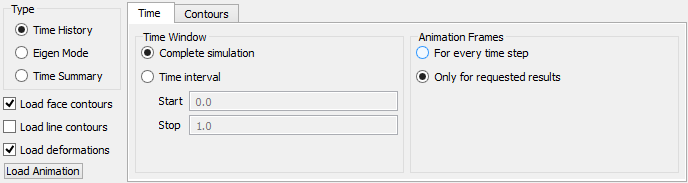
\includegraphics[trim=122 0 0 0,clip,width=0.82\textwidth]{\ReferenceImg/prp/animation-1}}
  \put(75,68){\Bullet{1}}
  \put(230,68){\Bullet{2}}
\end{picture}

\begin{bulletlist}
\item{\sl Time Window} --
  You can choose to display the entire duration of the simulation or a specific
  time interval. If you select {\sl Time Interval}, enter values for the
  interval's {\sl Start} and {\sl Stop} time.

\item{\sl Animation Frames} --
  These options are useful if you specified different time steps
  for the dynamics simulation and the stress recovery calculation
  (see \refSection{stress-recovery-options}{Stress recovery options}).
  Enabling {\sl For every time step} loads deformation results and color contour
  values for all the time steps calculated within the time window specified.
\end{bulletlist}

\Note{Enabling {\rm For every time step} shows continuous motion.
  However, the stress color contours may flash on and off if the calculation
  intervals are different. If you select {\rm Only for requested results},
  then only intervals shown are those at which the stress is calculated;
  both stress contours and motion appear continuous.}

\SubSubSection{Contours tab}{contours-tab}

If you selected {\sl Load face contours} and/or {\sl Load line contours} in the
Property Editor panel, you can display color contours on the mechanism assembly
during the animation (for {\sl Time History} and {\sl Time Summary} animations
only). You must then specify the values to be used for the color contours on
the {\sl Contours} tab (shown below) in the Property Editor panel,
before loading the animation.
The {\sl Contours} tab is not available for {\sl Eigen Mode} animation.

\noindent
\begin{picture}(282,90)
  \put(30,0){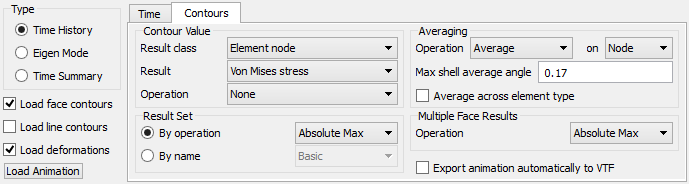
\includegraphics[trim=122 0 0 0,clip,width=0.82\textwidth]{\ReferenceImg/prp/animation-2}}
  \put(75,71) {\Bullet{1}}
  \put(68,29){\Bullet{2}}
  \put(210,71){\Bullet{3}}
  \put(228,29){\Bullet{4}}
  \put(274,3){\Bullet{5}}
\end{picture}

\vspace{-1mm}
\begin{bulletlist}
\item{\sl Contour Value} --
  These options are used to select the results that will be displayed
  as color contours.

  \begin{itemize}
  \subitem{\sl Result class} :
    This option allows selection of the FE entities for which you want to show
    color contours. You can select either nodes, elements (one single result for
    each element) or element nodes (one result for each node within an element).
    This selection controls the options for the {\sl Result} and {\sl Operation}
    settings (see below).
  \subitem{\sl Result} :
    This option allows you to specify which type of result to display in the
    animation: stress, strain, deformation, etc. The options available depend on
    the {\sl Result class} setting, and on the actual results currently
    available in the results database.
  \subitem{\sl Operation} :
    This option allows you to specify the scalar value to extract from the
    selected result, such as component selection, von Mises, principle values,
    and so on. The operations available depend on both the {\sl Result class}
    and {\sl Result} settings.
  \end{itemize}

  \EnumNote{There are two ways of animating some stress and strain measures.
    For instance, a von Mises stress animation may be set either by choosing
    {\rm Result $\rightarrow$ Stress} and
    {\rm Operation $\rightarrow$ von Mises}, or by choosing
    {\rm Result $\rightarrow$ von Mises stress} directly.
    The reason for this is the option to recover the desired derived
    stress/strain measures directly (see
    \refSection{stress-recovery-options}{Stress recovery options}).
    In the above example, if the entire stress tensor was recovered,
    the first animation definition would be correct.
    If only the von Mises stress measure was recovered,
    the second definition should be used.
    Choosing the wrong definition would leave an empty animation.}

\item{\sl Result Set} --
  These options allow you to select one of the named result sets for the
  {\sl Result class} (node, element, or element node) you selected.
  This setting is used to distinguish between multiple results for the specified
  FE entity, including results from different layers within an element (for
  example, top and bottom of a shell element), or multiple deformation results
  on a node (for example, mode shape deformations for different eigenmodes).

  \begin{itemize}
  \subitem{\sl By operation} :
    Enabling this option consolidates the entire result set of the same type
    using the selected operation. The options include {\sl Average},
    {\sl Maximum}, {\sl Minimum}, {\sl Max Difference}, and so on.
  \subitem{\sl By name} :
    Enabling this option allows you to load and display only the result sets
    with the specified name.
    Complete parts without such a result set will remain unchanged.
    Elements of a part without the result set will be rendered gray.
  \end{itemize}

\item{\sl Averaging} --
  The averaging options allow you to control how a continuous contour plot is
  obtained when the underlying results are discontinuous across the finite
  elements. They are available only when the selected {\sl Result class} is
  {\sl Element node} (see bullet 1 above).

  \begin{itemize}
  \subitem{\sl Operation} :
    Allows you to select the actual operation to use ({\sl Average}, {\sl Max},
    etc.), or select {\sl None} if averaging is not wanted.
  \subitem{\sl on} :
    Averaging on {\sl Node} calculates a single value for each node in the
    FE model, based on the selected {\sl Operation} and the values specified
    in the {\sl Contour Value} settings. Averaging on {\sl Element} calculates
    a single value for each element in the same way.
  \subitem{\sl Max shell average angle} :
    You can specify an angle above which the averaging between shells stops.
    The angle is used as a tolerance when comparing the globalized coordinate
    systems of the elements.
  \subitem{\sl Average across element type} :
    If enabled, Fedem averages the contour values across element type borders.
  \end{itemize}

\item{\sl Multiple Face Results} --
  This option enables you to specify the averaging behavior across elements
  that interface on a surface (such as stacking of elements with the same size
  and shape but different thicknesses). You can either specify an averaging
  operation, or select a named element group containing the result to be shown.

  \EnumTip{Contour data is only loaded for visible elements.
    This means that you can select which of the multiple face results you want
    to show by hiding appropriate elements.}

\item{\sl Export animation automatically to VTF} --
  When this toggle is enabled, the selected animation will be exported to a
  VTF-file after a batch stress recovery (see
  \refSection{batch-solving-trough-the-user-interface}
             {Batch solving trough the User Interface})
  if the command-line option {\tt-exportAnimation} is specified.
  The name on the VTF-file derived from the {\sl Description} of the animation.
\end{bulletlist}

\SubSubSection{Eigen Modes tab}{eigen-modes-tab}

If you selected {\sl Eigen Mode} as the animation type in the Property Editor
panel, you can animate the rigid body mode shapes calculated by Fedem while
solving the dynamics. If the Mode Shape Recovery analysis is performed, it is
also possible to include part deformations associated with the eigenmode in the
animation. You may also animate part mode shapes computed during the FE model
reduction if the {\sl Expand mode shape} toggle in the
\protect\hyperlink{reduction-options-tab}{\sl Reduction Options tab}
was on (see \refSection{part-properties}{Part properties"}).

To animate mode shapes, you must specify the settings on the {\sl Eigen Modes}
tab (shown below) in the Property Editor panel, before loading the animation.
This tab is not available for {\sl Time History} and {\sl Time Summary}
animations.

\noindent
\begin{picture}(282,92)
  \put(30,0){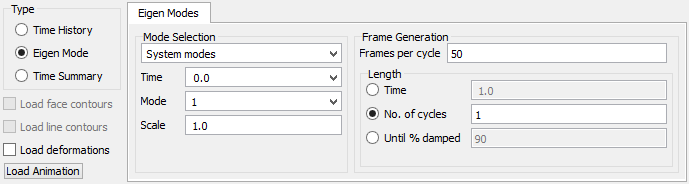
\includegraphics[trim=122 0 0 0,clip,width=0.82\textwidth]{\ReferenceImg/prp/animation-3}}
  \put(75,67){\Bullet{1}}
  \put(196,67){\Bullet{2}}
\end{picture}

\begin{bulletlist}
\item{\sl Mode Selection} --
  These options allow you to select the mode type, time step or part,
  mode number, and a scale factor for the animation:

  \begin{itemize}
  \subitem
    Select between {\sl System modes}, {\sl Component modes of part} and
    {\sl Free-free modes of reduced part} from the first pull-down menu.
  \subitem{\sl Time} :
    If you selected {\sl System modes}, this pull-down menu lists the times at
    which an Eigenmode solution is specified in the Dynamics Solverdialog box
    (see \refSubSection{eigenmode-tab}{Eigenmode tab}
    {dynamics-solver-advanced-mode}).
  \subitem{\sl Part} :
    If you selected either {\sl Component modes of part} or
    {\sl Free-free modes of reduced part}, this pull-down menu lists all parts
    in the model. It also have an entry {\sl(All parts)} to enable simultaneous
    part mode shape animations for all parts. (See
    \refSection{visualization-of-eigenmode-shapes-from-the-model-reduction}
               {Visualization of eigenmode shapes from the model reduction}
    to learn more on such mode shape visualization.)
  \subitem{\sl Mode} :
    This pull-down menu shows either the modes specified in the Dynamics Solver
    dialog box (see \refSubSection{eigenmode-tab}{Eigenmode tab}
    {dynamics-solver-advanced-mode}), the component mode numbers (see
    \refSubSection{reduction-options-tab}{Reduction Options tab}
                  {part-properties})
    or the free-free mode numbers for the reduced part,
    depending on the selected  mode type in the first pull-down menu in the
    {\sl Mode Selection} frame.
  \subitem{Scale} : You can
    specify a scale factor to exaggerate the mode shapes during the animation.
  \end{itemize}

\EnumNote{The default {\rm Scale} setting (1.0) implies that the maximum
  amplitude of the mode shape is equal to the length scale used to model
  the mechanism. Therefore, if the length-span of the model is not 1.0,
  it might be necessary to adjust this setting in order to obtain an
  appropriate deformation scale.}

\item{\sl Frame Generation} --
  These options allow you to set the number of animation frames and the
  duration of the animation:

  \begin{itemize}
  \subitem{\sl Frames per cycle} :
    Entering a higher value increases the continuity of the animated motion.
  \subitem{\sl Length} :
    You can specify either a {\sl Time}, {\sl No.\ of cycles},
    or {\sl Until \% damped} to limit the duration of the animation.
    These fields are available only for {\sl System modes.}
    For {\sl Component modes of part} and {\sl Free-free modes of reduced part},
    the duration of the animation will always be equal one full cycle.
  \end{itemize}

\EnumNote{The {\rm Until \% Damped} option is relevant only if
  a damped eigenmode solution was performed (see
  \refSubSection{eigenmode-tab}{Eigenmode tab}{dynamics-solver-advanced-mode}).}
\end{bulletlist}

\Note{When animating eigenmode shapes, the time that runs in the upper right
  corner of the {\rm Modeler} view is in the range $[0,nT]$ where $T$ is the
  period ($=1/{\rm eigenfrequency}$) and $n$ is the number of cycles that are
  animated (usually $n=1$ for free vibrations and $n>1$ for damped vibrations).}


\subsection{Available animation results}

The results available for animation depend on the solvers that have been run and
their settings. For an indication of which results that could be available,
use the Result File Browser
(see \refSection{result-file-browser}{Result File Browser}).

\Tip{The heading of the \File{.frs} files (Fedem Result File) is readable
  and could give valuable information in some cases.}

If an animation is loaded without the contour results in question being present,
the legend text will display a question mark for the max and min values,
and no contour colors will appear.

Most of the results that can be viewed in a contour animation are produced
during the Stress Recovery analysis. All {\sl Element Node} and {\sl Node}
results (selected in the {\sl Result Class} pull-down menu) are currently
produced by the Stress Recovery analysis. All {\sl Element} results, however,
are produced by the Strain Coat Recovery Summary analysis,
and include the following quantities:

\begin{itemize}
\item Max principal stress
\item Max principal strain
\item Max shear stress
\item Max shear strain
\item Max von Mises stress
\item Max von Mises strain
\item Maximum stress range
\item Maximum strain range
\item Mean biaxiality
\item Biaxiality standard deviation
\item Most popular angle
\item Angle Spread
\item Damage
\item Life (repeats)
\item Life (equnits)
\end{itemize}

\subsubsection{Interpretation of shear strains in contour plots}

The stress- or strain state at a point in the model can be represented as
a second-order tensor in a mathematical setting, i.e., in 2D we have
$$
\mbox{\boldmath$\sigma$} \;= \left[
  \begin{array}{cc}
    \sigma_{xx} & \sigma_{xy} \\
    \sigma_{yx} & \sigma_{yy}
  \end{array}
  \right] \quad\text{and}\quad
\mbox{\boldmath$\epsilon$} \;= \left[
  \begin{array}{cc}
    \epsilon_{xx} & \epsilon_{xy} \\
    \epsilon_{yx} & \epsilon_{yy}
  \end{array}\right]
$$
where equilibrium in angular momentum requires $\sigma_{xy}=\sigma_{yx}$.
The strain components are defined as $\epsilon_{ij}=\frac{1}{2}(u_{i,j}+u_{j,i})$,
where $u$ is the deformation and the indices $i$ and $j$ both run through
$x$ and $y$ (or $x$, $y$ and $z$ in 3D). The advantage of this representation
is that computation of von Mises and principal quantities can be performed using
the same piece of code for stress and strain thereby making the implementation
more general and robust.

An alternative representation (more common to engineers) is by means of
the stress and strain vectors, i.e., in 2D we have
$$
\mbox{\boldmath$\sigma$} \;= \left[
  \begin{array}{c}
    \sigma_{xx} \\
    \sigma_{yy} \\
    \sigma_{xy}
  \end{array}
  \right] \quad\mbox{and}\quad
\mbox{\boldmath$\epsilon$} \;= \left[
  \begin{array}{c}
    \epsilon_{xx} \\
    \epsilon_{yy} \\
    \gamma_{xy}
  \end{array}
  \right]
$$
where $\gamma_{xy}=\epsilon_{xy}+\epsilon_{yx}=\frac{1}{2}(u_{x,y}+ u_{y,x})$
and thus $\gamma_{xy}=2\epsilon_{xy}$.

The results from a Stress Recovery analysis that may be visualized in an
animation are based on the tensorial strain representation, i.e.,
the shear strain components (including Max Shear) are equivalent to the
$\epsilon_{xy}$-term and not $\gamma_{xy}$. However, the Max Shear strain
quantity computed from the Strain Coat Recovery Summary analysis is currently
based on the vector representation so that it will be twice as large as the
equivalent quantity from the stress recovery analysis. It is important to be
aware of this distinction when using that particular result quantity.

\subsubsection{Stress and strain range quantities}

The maximum stress- and strain range quantities computed in the Strain Coat
Recovery are derived from the principal value history at each point.
This computation is performed in a similar manner as for the
{\sl Most popular angle} and {\sl Angle Spread} quantities.
That is, the directions of the maximum (and minimum) principal values,
in terms of the in-plane angle from the $X$-axis of the stress coordinate
system, are used to divide the principal stress states into a discrete number
of {\sl bins} for each stress point. The principal stress values at a certain
time is then assigned to one such bin depending on its angle, and the range for
each such bin is computed as the difference between the highest and the lowest
value over the whole time history. The range value presented in the
{\sl Time Summary} animations is then selected from the bin having the largest
computed range value.


\SubSection{Performance of animation loading}{performance-of-animation-loading}

It is important to be aware that the performance of the animation
loading is highly dependent upon the animation settings, especially when
working with large FE-models ($>30.000$ elements).

Memory usage is the most crucial point, and can be reduced to 1/3 when
using the better options mentioned below.

The significant parameters are in order of decreasing importance:

\begin{enumerate}
\item
  {\sl Result Set} selection is {\sl By operation} or {\sl By name}.
  ({\sl By name} is better.)
\item
  {\sl Load face contours} and/or {\sl Load line contours} are toggled.
  ({\sl Only load face contours} is better.)
\item
  {\sl Averaging} is turned on or off.
  ({\sl No averaging} is better.)
\end{enumerate}

The number of elements visible when the animation is loaded is also
important because result values will only be loaded for visible element
faces. This means that you can load contour data for one group at a time
if loading data for the complete part is too memory and time consuming.


%%%%%%%%%%%%%%%%%%%%%%%%%%%%%%%%%%%%%%%%%%%%%%%%%%%%%%%%%%%%%%%%%%%%%%%%%%%%%%%%
\Section{Viewing animations}{viewing-animations}

When an animation is loaded, you can use several tools to view and explore the
data you have loaded. The {\sl Modeler} view will display some additional
features and the Animation Control dialog box will be made available.
These views are shown in the figure below.

\medskip\noindent
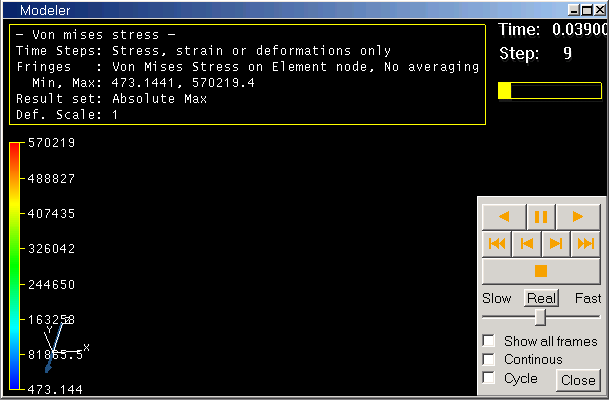
\includegraphics[height=0.47\textwidth]{Figures/AnimationWindow} \hfill
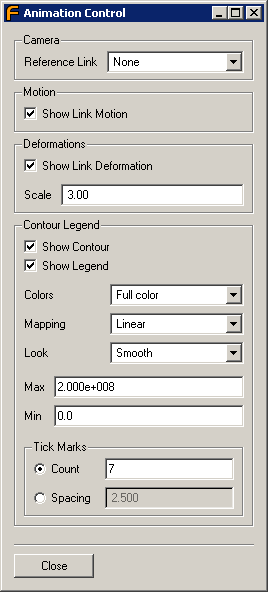
\includegraphics[height=0.47\textwidth]{Figures/Dialogs/7-AnimationControl}
\begin{picture}(343,0)
  \put(-14,145){\Bullet{1}}
  \put(-14,100){\Bullet{2}}
  \put(243,140){\Bullet{3}}
  \put(243, 80){\Bullet{4}}
  \put(255,155){\Bullet{5}}
\end{picture}

\begin{bulletlist}
\item{\sl Legend text} --
  Displays information regarding the loaded animation.
\item{\sl Legend bar} --
  Indicates the color assigned to each contour value.
\item{\sl Time step information} --
  Displays the time and the time step number for the current frame
  along with a progress bar.
\item{\sl Play panel} --
  This panel is used to control how the animation is run.
\item{\sl Animation Control} --
  This dialog box features options to control several aspects of the animation,
  including deformation scale and contour legend domain.
\end{bulletlist}

\clearpage


\SubSection{Play panel}{play-panel}

\begin{wrapfigure}[11]{r}{0.4\textwidth}
  \vspace{-6mm}
  \begin{picture}(103,158)
    \put(0,0){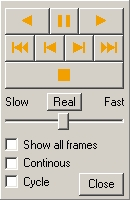
\includegraphics[width=0.3\textwidth]{Figures/7-PlayPanel}}
    \put(-2,145){\Bullet{1}}
    \put(40,145){\Bullet{2}}
    \put(80,145){\Bullet{3}}
    \put(-4,121){\Bullet{4}}
    \put(30,121){\Bullet{5}}
    \put(50,121){\Bullet{6}}
    \put(86,121){\Bullet{7}}
    \put(10,95){\Bullet{8}}
    \put(20,58){\Bullet{9}}
    \put(-9,38){\BBullet{10}}
    \put(-9,24){\BBullet{11}}
    \put(-9,10){\BBullet{12}}
    \put(90,9){\BBullet{13}}
  \end{picture}
\end{wrapfigure}

The Play panel (shown to the right) is displayed in the lower-right corner
of the {\sl Modeler} view when an animation is loaded.

\begin{bulletlist}
\item{\sl Reverse Play}
\item{\sl Pause Play}
\item{\sl Forward Play}
\item{\sl Beginning}
\item{\sl Rewind by Frame}
\item{\sl Forward by Frame}
\item{\sl End}
\item{\sl Stop Play}
\end{bulletlist}

%Must restart the bullet list, to avoid the wrapfigure screws up.
\begin{bulletlist}
   \setcounter{enumi}{8}
 \item{\sl Speed} slider --
   You can adjust the speed of the animation by moving the slider to the right
   or left. You can also click the \textbf{Real} button to return the speed to
   ``real time''.

   \EnumNote{At faster speeds, Fedem may skip frames in order to maintain
     animation speed at the level you have specified.}
 \item{\sl Show all frames} --
   This option forces Fedem to show all the frames loaded,
   ignoring the {\sl Speed} setting if necessary.
 \item{\sl Continuous} --
   This option allows you to play the animation repeatedly until you click the
   {\sl Stop Play} button.
 \item{\sl Cycle} --
   Enables playing the animation in {\sl Forward Play}  mode until it reaches
   the end, then plays it in {\sl Reverse Play} mode.
 \item\textbf{Close} --
   This button closes the Play panel and ends the current animation session.
\end{bulletlist}

\Note{The Play panel does not appear if the animation consists of a single frame
  (e.g., {\rm Time Summary} animation with results from a Strain Coat Recovery).
  To close such an animation, you have to select \textbf{End Animation Session}
  from the \textbf{Results} menu, or type \textbf{Ctrl}+\textbf{X}.}

\clearpage


\SubSection{Animation controls}{animation-controls}

\begin{wrapfigure}[16]{r}{0.37\textwidth}
  \vspace{-5mm}
  \begin{picture}(127,260)
    \put(0,0){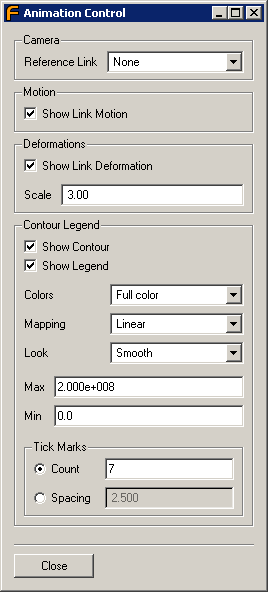
\includegraphics[width=0.37\textwidth]{Figures/Dialogs/7-AnimationControl}}
    \put(-5,255){\Bullet{1}}
    \put(-5,230){\Bullet{2}}
    \put(-5,205){\Bullet{3}}
    \put(-5,167){\Bullet{4}}
    \put(-267,237){
\includegraphics[width=7mm]{Figures/Icons/animationControls}}
  \end{picture}
\end{wrapfigure}

Once an animation is loaded, you can open the Animation Control dialog box by
selecting \textbf{Show Animation Controls...} on the \textbf{Tools} menu.
The Animation Control dialog box is opened as shown to the right.
Changes made to settings here are instantaneously applied to the animation.

\begin{bulletlist}
\item{\sl Camera} --
  Enables the selection of reference part for the camera movement. See also
  \protect\hyperlink{camera-reference-part}{\sl"Camera reference part"} below.
\item{\sl Motion} --
  Enables display of rigid body motion of the mechanism.
\item{\sl Deformations} --
  Enables display of part deformations scaled (exaggerated) by the {\sl Scale}
  factor you specify. Applies to time history animations only
  (i.e., not on eigenmode deformations).
\item{\sl Contour Legend} -- \newline
  These options enable you to customize the Contour Legend, and how the result
  numbers are converted to colors:

  \begin{itemize}
  \subitem{\sl Show Contour} : Enables the
    display of contour contours on the mechanism during the animation.
  \subitem{\sl Show Legend} :
    Enables display of the Contour Legend bar in the {\sl Modeler} view.
  \subitem{\sl Colors} :
    The type of Color mapping used for the color contour, e.g.,
    Full Color or Red Blue. See also
    \refSubSection{color-mappings}{Color mappings}{contour-legend-control}.
  \subitem{Mapping} :
    {\sl Linear} divides color increments linearly and
    {\sl Log10} divides color increments on a logarithmic scale.
  \subitem{Look} :
    Either {\sl Smooth} or {\sl Discrete}.
  \subitem{\sl Max/Min} :
    You can set a maximum and minimum value to show on the Contour Legend.
    See also \refSubSection{contour-value-domain-control}
    {Contour value domain control}{contour-legend-control}.
  \subitem{\sl Tick Marks} :
    You can select {\sl Count} (number of ticks) or {\sl Spacing}
    (difference between tick marks) and specify a value to change
    the tick marks on the legend.
    See also \refSubSection{tick-marks}{Tick marks}{contour-legend-control}.
  \end{itemize}
  \EnumNote{Discrete contours should only be selected when each face in the
    model has one single color, for example when showing single element results
    or results averaged on elements.}
\end{bulletlist}

\SubSubSection{Camera reference part}{camera-reference-part}

When viewing an animation, it is possible to make the camera follow the motion
of a part in the model. This is useful if some part of your model moves far
during the simulation. To do this, selecting the part to follow in the
{\sl Reference Part} pull-down menu in the Animation Control dialog box.


\SubSection{Contour legend control}{contour-legend-control}

\SubSubSection{Color mappings}{color-mappings}

The drop-down menu labeled {\sl Colors} in the Animation Control dialog box
enables the selection of different color mappings for the contour values.
The different color mappings map the contour values differently.
This concerns values above, within and below the legend domain.
They also show undefined results differently.

There are currently four color mappings available:

\begin{enumerate}
  \setlength\itemsep{3mm}

\item{\sl Full Color} --
  This is the default mapping and is a common way to display structural results.

  \begin{tabular}{ | m{4.0cm} | m{6cm} | }
    \hline
    Values               & Color \\
    \hline\hline
    Above legend domain  & Red \\
    \hline
    Within legend domain & Blue-Cyan-Green-Yellow-Orange-Red \\
    \hline
    Below legend domain  & Blue \\
    \hline
    Undefined            & Gray \\
    \hline
\end{tabular}

\item{\sl Full Color B/W Limits} --
  This is a mapping used to show what is within and outside the legend domain.

  \begin{tabular}{ | m{4.0cm} | m{6cm} | }
    \hline
    Values               & Color \\
    \hline\hline
    Above legend domain  & White \\
    \hline
    Within legend domain & Blue-Cyan-Green-Yellow-Orange-Red \\
    \hline
    Below legend domain  & Black \\
    \hline
    Undefined            & Gray \\
    \hline
  \end{tabular}

\item{\sl Full Color Clipped Limits} --
  This is a mapping that is useful when you want a quick overview of the few
  elements in a big complex model with results within a certain (narrow) value
  domain. It renders all elements outside the domain transparent, i.e.,
  the elements within the domain will be the only ones visible.

  \begin{tabular}{ | m{4.0cm} | m{6cm} | }
    \hline
    Values               & Color \\
    \hline\hline
    Above legend domain  & Invisible \\
    \hline
    Within legend domain & Blue-Cyan-Green-Yellow-Orange-Red \\
    \hline
    Below legend domain  & Invisible \\
    \hline
    Undefined            & Invisible \\
    \hline
  \end{tabular}

\item{\sl Red Blue} --
  This is a mapping useful when you want the interpolation of colors within one
  element-face to be strictly consistent with the contour legend.
  Because of limitations in the 3D graphics hardware, interpolations of colors
  within one face will be linear. That makes the normal full color mapping
  inconsistent within one face if the different nodes in the element-face
  have values that map to colors separated by one or more colors in the legend
  domain.

  \begin{tabular}{ | m{4.0cm} | m{3cm} | }
    \hline
    Values               & Color \\
    \hline\hline
    Above legend domain  & Red \\
    \hline
    Within legend domain & Blue-Red \\
    \hline
    Below legend domain  & Blue \\
    \hline
    Undefined            & Gray \\
    \hline
  \end{tabular}

\end{enumerate}

\SubSubSection{Contour value domain control}{contour-value-domain-control}

The {\sl Max} and {\sl Min} fields in the Animation Control dialog box are used
to control the domain of the color legend. The default value is 0.0 for both.
In this case Fedem uses the maximum and minimum values of the loaded contour
results.

The {\sl Max}/{\sl Min} fields can also be used to ``flip'' the legend scale in
order to show the least values as ``red'' or ``worst''. To do this,
simply enter the worst value in the field labeled {\sl Max}, and the best value
in the field labeled {\sl Min}, ignoring the relative size of the numbers.

When using a logarithmic mapping of the contour values, make sure that both the
max and min values are above zero. If not, Fedem will not be able to calculate
valid contour colors ($\log(x)$ does not exist when $x\leq0$).

\SubSubSection{Tick marks}{tick-marks}

There are two ways to control the tick marks on the color legend.
Either by setting the number of tick marks wanted, or by setting the spacing
between the tick marks.

When selecting Count, Fedem will distribute the given number of tick marks
evenly in the value domain.

When selecting Spacing, Fedem will set tick marks with the given spacing between
them, starting at the first complete multiple of the spacing value.
When using a logarithmic mapping, the supplied value is multiplied with the
decade in question.

\Tip{When using logarithmic mapping, choose Spacing as tick mark distribution,
  and either 1, 2.5, 5 or 10 as spacing value.}

\subsubsection{Interpreting fatigue results}

When calculating fatigue results, some of the elements are rejected because they
have near infinite life/zero damage. These elements are excluded form the
max/min calculations done by Fedem when reading the results.
Fedem assigns them a reference value that make them show up as little damage or
high life when using the ordinary Full Color legend mapping.
If {\sl Full Color B/W limits} are used, those elements will show up as Black
(below legend domain) if plotting damage, or White (above legend domain) if
plotting life. {\sl If using Full Color Clipped Limits} all these elements will
be removed from the display, leaving the interesting elements in the display.

The reference values Fedem uses are:

\begin{itemize}
\item Damage: $1\times10^{-20}$
\item Log Damage: $-20$
\item All life plots (repeats/equnits/Log): $1\times10^{20}$
\end{itemize}


\SubSection{Exporting animations}{exporting-animations}

The loaded animation can be exported to the mpeg-1, mpeg-2 and avi formats for
viewing in an external viewer. Avi export is available on Windows only.

The animation you have loaded forms the basis for the exported animation.
Through a simple dialog box,
you will be able to control the speed of the animation.

\clearpage
\begin{wrapfigure}[11]{r}{0.45\textwidth}
  \begin{picture}(200,120)
    \put(0,0){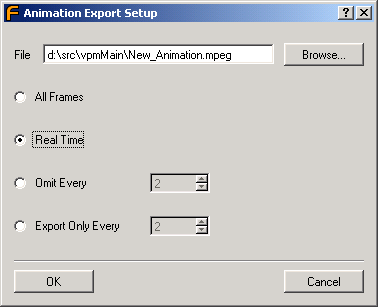
\includegraphics[width=0.45\textwidth]{Figures/Dialogs/7-ExportAnimation}}
    \put(105,98){\Bullet{1}}
    \put(35,79){\Bullet{2}}
    \put(35,62){\Bullet{3}}
    \put(35,45){\Bullet{4}}
    \put(47,27){\Bullet{5}}
  \end{picture}
\end{wrapfigure}

To start export, go to the text{File} menu, select \textbf{Export} and then
\textbf{Export Animation...} The Animation Export Setup dialog box
(shown to the right) will then be opened:

\begin{bulletlist}
\item{\sl File} --
  Either type in the file name you or click the \textbf{Browse...} button box.
  If you type the the given extension will decide which format the animation
  will be exported to. The default is to save the animation to model file root,
  with same name as in animation's description.
  The default file format is mpeg-1.
\end{bulletlist}

%Must restart the bullet list, to avoid the wrapfigure screws up.
\begin{bulletlist}
   \setcounter{enumi}{1}
\item{\sl All Frames} --
  The animation will be exported "as is". The speed of the exported animation
  will depend solely on the simulation's time step size.
\item{\sl Real Time} --
  The animation will be exported so that one second movie time corresponds to
  one second of simulation time. Note that the animation's frame rate is 30 Hz,
  so this will be an approximation.
\item{\sl Omit Every} --
  Every {\sl n}$^{th}$ frame will be omitted when exported.
\item{Export Only Every} --
  Most useful when you have solved using small time steps,
  and want finer control over what you export.
\end{bulletlist}

\subsubsection{Hints and tricks}

When exporting to mpeg, the {\sl mpeg-1} format produces smaller files than the
{\sl mpeg-2 elecard} format, and the quality is approximately the same.
For best result, use black background.
It seems that the MS Windows Media Player has problems playing the exported
mpeg files on some machines. If you discover this, you can try to play the
animations with the Elecard mpeg player instead
(\href{https://www.elecard.com/}{\sl elecard.com}).
Also note that the Windows Media Player has a size limit of 720x480 pixels.

If you are working on Windows, we recommend exporting to {\sl avi} format.
This export is faster and also produces better quality. When you
export to {\sl avi}, a dialog box will pop up where you can set up
which codec to use and settings for this codec. Be aware that some
codecs may not work, this is dependent on your system configuration.
The codecs that seem to have the best success rate is {\sl MS Video 1},
{\sl Cinepak by Radius}, and the \href{https://www.divx.com/}{\sl Divx codec}.
If you don't have a DivX codec installed on your machine,
you can get it from the DivX home page.
